\documentclass{report}
\usepackage{amssymb}
\usepackage{amsmath} % Per le formule matematiche
\usepackage{tikz}    % Per i diagrammi
\usetikzlibrary{trees}

%%%%%%%%%%%%%%%%%%%%%%%%%%%%%%%%%
% PACKAGE IMPORTS
%%%%%%%%%%%%%%%%%%%%%%%%%%%%%%%%%


\usepackage[tmargin=2cm,rmargin=1in,lmargin=1in,margin=0.85in,bmargin=2cm,footskip=.2in]{geometry}
\usepackage{amsmath,amsfonts,amsthm,amssymb,mathtools}
\usepackage[varbb]{newpxmath}
\usepackage{xfrac}
\usepackage[makeroom]{cancel}
\usepackage{mathtools}
\usepackage{bookmark}
\usepackage{enumitem}
\usepackage{hyperref,theoremref}
\hypersetup{
	pdftitle={Assignment},
	colorlinks=true, linkcolor=doc!90,
	bookmarksnumbered=true,
	bookmarksopen=true
}
\usepackage[most,many,breakable]{tcolorbox}
\usepackage{xcolor}
\usepackage{varwidth}
\usepackage{varwidth}
\usepackage{etoolbox}
%\usepackage{authblk}
\usepackage{nameref}
\usepackage{multicol,array}
\usepackage{tikz-cd}
\usepackage[ruled,vlined,linesnumbered]{algorithm2e}
\usepackage{comment} % enables the use of multi-line comments (\ifx \fi) 
\usepackage{import}
\usepackage{xifthen}
\usepackage{pdfpages}
\usepackage{transparent}

\newcommand\mycommfont[1]{\footnotesize\ttfamily\textcolor{blue}{#1}}
\SetCommentSty{mycommfont}
\newcommand{\incfig}[1]{%
    \def\svgwidth{\columnwidth}
    \import{./figures/}{#1.pdf_tex}
}

\usepackage{tikzsymbols}
\renewcommand\qedsymbol{$\Laughey$}


%\usepackage{import}
%\usepackage{xifthen}
%\usepackage{pdfpages}
%\usepackage{transparent}


%%%%%%%%%%%%%%%%%%%%%%%%%%%%%%
% SELF MADE COLORS
%%%%%%%%%%%%%%%%%%%%%%%%%%%%%%



\definecolor{myg}{RGB}{56, 140, 70}
\definecolor{myb}{RGB}{45, 111, 177}
\definecolor{myr}{RGB}{199, 68, 64}
\definecolor{mytheorembg}{HTML}{F2F2F9}
\definecolor{mytheoremfr}{HTML}{00007B}
\definecolor{mylenmabg}{HTML}{FFFAF8}
\definecolor{mylenmafr}{HTML}{983b0f}
\definecolor{mypropbg}{HTML}{f2fbfc}
\definecolor{mypropfr}{HTML}{191971}
\definecolor{myexamplebg}{HTML}{F2FBF8}
\definecolor{myexamplefr}{HTML}{88D6D1}
\definecolor{myexampleti}{HTML}{2A7F7F}
\definecolor{mydefinitbg}{HTML}{E5E5FF}
\definecolor{mydefinitfr}{HTML}{3F3FA3}
\definecolor{notesgreen}{RGB}{0,162,0}
\definecolor{myp}{RGB}{197, 92, 212}
\definecolor{mygr}{HTML}{2C3338}
\definecolor{myred}{RGB}{127,0,0}
\definecolor{myyellow}{RGB}{169,121,69}
\definecolor{myexercisebg}{HTML}{F2FBF8}
\definecolor{myexercisefg}{HTML}{88D6D1}


%%%%%%%%%%%%%%%%%%%%%%%%%%%%
% TCOLORBOX SETUPS
%%%%%%%%%%%%%%%%%%%%%%%%%%%%

\setlength{\parindent}{1cm}
%================================
% THEOREM BOX
%================================

\tcbuselibrary{theorems,skins,hooks}
\newtcbtheorem[number within=section]{Theorem}{Theorem}
{%
	enhanced,
	breakable,
	colback = mytheorembg,
	frame hidden,
	boxrule = 0sp,
	borderline west = {2pt}{0pt}{mytheoremfr},
	sharp corners,
	detach title,
	before upper = \tcbtitle\par\smallskip,
	coltitle = mytheoremfr,
	fonttitle = \bfseries\sffamily,
	description font = \mdseries,
	separator sign none,
	segmentation style={solid, mytheoremfr},
}
{th}

\tcbuselibrary{theorems,skins,hooks}
\newtcbtheorem[number within=chapter]{theorem}{Theorem}
{%
	enhanced,
	breakable,
	colback = mytheorembg,
	frame hidden,
	boxrule = 0sp,
	borderline west = {2pt}{0pt}{mytheoremfr},
	sharp corners,
	detach title,
	before upper = \tcbtitle\par\smallskip,
	coltitle = mytheoremfr,
	fonttitle = \bfseries\sffamily,
	description font = \mdseries,
	separator sign none,
	segmentation style={solid, mytheoremfr},
}
{th}


\tcbuselibrary{theorems,skins,hooks}
\newtcolorbox{Theoremcon}
{%
	enhanced
	,breakable
	,colback = mytheorembg
	,frame hidden
	,boxrule = 0sp
	,borderline west = {2pt}{0pt}{mytheoremfr}
	,sharp corners
	,description font = \mdseries
	,separator sign none
}

%================================
% Corollery
%================================
\tcbuselibrary{theorems,skins,hooks}
\newtcbtheorem[number within=section]{Corollary}{Corollary}
{%
	enhanced
	,breakable
	,colback = myp!10
	,frame hidden
	,boxrule = 0sp
	,borderline west = {2pt}{0pt}{myp!85!black}
	,sharp corners
	,detach title
	,before upper = \tcbtitle\par\smallskip
	,coltitle = myp!85!black
	,fonttitle = \bfseries\sffamily
	,description font = \mdseries
	,separator sign none
	,segmentation style={solid, myp!85!black}
}
{th}
\tcbuselibrary{theorems,skins,hooks}
\newtcbtheorem[number within=chapter]{corollary}{Corollary}
{%
	enhanced
	,breakable
	,colback = myp!10
	,frame hidden
	,boxrule = 0sp
	,borderline west = {2pt}{0pt}{myp!85!black}
	,sharp corners
	,detach title
	,before upper = \tcbtitle\par\smallskip
	,coltitle = myp!85!black
	,fonttitle = \bfseries\sffamily
	,description font = \mdseries
	,separator sign none
	,segmentation style={solid, myp!85!black}
}
{th}


%================================
% LENMA
%================================

\tcbuselibrary{theorems,skins,hooks}
\newtcbtheorem[number within=section]{Lenma}{Lenma}
{%
	enhanced,
	breakable,
	colback = mylenmabg,
	frame hidden,
	boxrule = 0sp,
	borderline west = {2pt}{0pt}{mylenmafr},
	sharp corners,
	detach title,
	before upper = \tcbtitle\par\smallskip,
	coltitle = mylenmafr,
	fonttitle = \bfseries\sffamily,
	description font = \mdseries,
	separator sign none,
	segmentation style={solid, mylenmafr},
}
{th}

\tcbuselibrary{theorems,skins,hooks}
\newtcbtheorem[number within=chapter]{lenma}{Lenma}
{%
	enhanced,
	breakable,
	colback = mylenmabg,
	frame hidden,
	boxrule = 0sp,
	borderline west = {2pt}{0pt}{mylenmafr},
	sharp corners,
	detach title,
	before upper = \tcbtitle\par\smallskip,
	coltitle = mylenmafr,
	fonttitle = \bfseries\sffamily,
	description font = \mdseries,
	separator sign none,
	segmentation style={solid, mylenmafr},
}
{th}


%================================
% PROPOSITION
%================================

\tcbuselibrary{theorems,skins,hooks}
\newtcbtheorem[number within=section]{Prop}{Proposition}
{%
	enhanced,
	breakable,
	colback = mypropbg,
	frame hidden,
	boxrule = 0sp,
	borderline west = {2pt}{0pt}{mypropfr},
	sharp corners,
	detach title,
	before upper = \tcbtitle\par\smallskip,
	coltitle = mypropfr,
	fonttitle = \bfseries\sffamily,
	description font = \mdseries,
	separator sign none,
	segmentation style={solid, mypropfr},
}
{th}

\tcbuselibrary{theorems,skins,hooks}
\newtcbtheorem[number within=chapter]{prop}{Proposition}
{%
	enhanced,
	breakable,
	colback = mypropbg,
	frame hidden,
	boxrule = 0sp,
	borderline west = {2pt}{0pt}{mypropfr},
	sharp corners,
	detach title,
	before upper = \tcbtitle\par\smallskip,
	coltitle = mypropfr,
	fonttitle = \bfseries\sffamily,
	description font = \mdseries,
	separator sign none,
	segmentation style={solid, mypropfr},
}
{th}


%================================
% CLAIM
%================================

\tcbuselibrary{theorems,skins,hooks}
\newtcbtheorem[number within=section]{claim}{Claim}
{%
	enhanced
	,breakable
	,colback = myg!10
	,frame hidden
	,boxrule = 0sp
	,borderline west = {2pt}{0pt}{myg}
	,sharp corners
	,detach title
	,before upper = \tcbtitle\par\smallskip
	,coltitle = myg!85!black
	,fonttitle = \bfseries\sffamily
	,description font = \mdseries
	,separator sign none
	,segmentation style={solid, myg!85!black}
}
{th}



%================================
% Exercise
%================================

\tcbuselibrary{theorems,skins,hooks}
\newtcbtheorem[number within=section]{Exercise}{Exercise}
{%
	enhanced,
	breakable,
	colback = myexercisebg,
	frame hidden,
	boxrule = 0sp,
	borderline west = {2pt}{0pt}{myexercisefg},
	sharp corners,
	detach title,
	before upper = \tcbtitle\par\smallskip,
	coltitle = myexercisefg,
	fonttitle = \bfseries\sffamily,
	description font = \mdseries,
	separator sign none,
	segmentation style={solid, myexercisefg},
}
{th}

\tcbuselibrary{theorems,skins,hooks}
\newtcbtheorem[number within=chapter]{exercise}{Exercise}
{%
	enhanced,
	breakable,
	colback = myexercisebg,
	frame hidden,
	boxrule = 0sp,
	borderline west = {2pt}{0pt}{myexercisefg},
	sharp corners,
	detach title,
	before upper = \tcbtitle\par\smallskip,
	coltitle = myexercisefg,
	fonttitle = \bfseries\sffamily,
	description font = \mdseries,
	separator sign none,
	segmentation style={solid, myexercisefg},
}
{th}

%================================
% EXAMPLE BOX
%================================

\newtcbtheorem[number within=section]{Example}{Example}
{%
	colback = myexamplebg
	,breakable
	,colframe = myexamplefr
	,coltitle = myexampleti
	,boxrule = 1pt
	,sharp corners
	,detach title
	,before upper=\tcbtitle\par\smallskip
	,fonttitle = \bfseries
	,description font = \mdseries
	,separator sign none
	,description delimiters parenthesis
}
{ex}

\newtcbtheorem[number within=chapter]{example}{Example}
{%
	colback = myexamplebg
	,breakable
	,colframe = myexamplefr
	,coltitle = myexampleti
	,boxrule = 1pt
	,sharp corners
	,detach title
	,before upper=\tcbtitle\par\smallskip
	,fonttitle = \bfseries
	,description font = \mdseries
	,separator sign none
	,description delimiters parenthesis
}
{ex}

%================================
% DEFINITION BOX
%================================

\newtcbtheorem[number within=section]{Definition}{Definition}{enhanced,
	before skip=2mm,after skip=2mm, colback=red!5,colframe=red!80!black,boxrule=0.5mm,
	attach boxed title to top left={xshift=1cm,yshift*=1mm-\tcboxedtitleheight}, varwidth boxed title*=-3cm,
	boxed title style={frame code={
					\path[fill=tcbcolback]
					([yshift=-1mm,xshift=-1mm]frame.north west)
					arc[start angle=0,end angle=180,radius=1mm]
					([yshift=-1mm,xshift=1mm]frame.north east)
					arc[start angle=180,end angle=0,radius=1mm];
					\path[left color=tcbcolback!60!black,right color=tcbcolback!60!black,
						middle color=tcbcolback!80!black]
					([xshift=-2mm]frame.north west) -- ([xshift=2mm]frame.north east)
					[rounded corners=1mm]-- ([xshift=1mm,yshift=-1mm]frame.north east)
					-- (frame.south east) -- (frame.south west)
					-- ([xshift=-1mm,yshift=-1mm]frame.north west)
					[sharp corners]-- cycle;
				},interior engine=empty,
		},
	fonttitle=\bfseries,
	title={#2},#1}{def}
\newtcbtheorem[number within=chapter]{definition}{Definition}{enhanced,
	before skip=2mm,after skip=2mm, colback=red!5,colframe=red!80!black,boxrule=0.5mm,
	attach boxed title to top left={xshift=1cm,yshift*=1mm-\tcboxedtitleheight}, varwidth boxed title*=-3cm,
	boxed title style={frame code={
					\path[fill=tcbcolback]
					([yshift=-1mm,xshift=-1mm]frame.north west)
					arc[start angle=0,end angle=180,radius=1mm]
					([yshift=-1mm,xshift=1mm]frame.north east)
					arc[start angle=180,end angle=0,radius=1mm];
					\path[left color=tcbcolback!60!black,right color=tcbcolback!60!black,
						middle color=tcbcolback!80!black]
					([xshift=-2mm]frame.north west) -- ([xshift=2mm]frame.north east)
					[rounded corners=1mm]-- ([xshift=1mm,yshift=-1mm]frame.north east)
					-- (frame.south east) -- (frame.south west)
					-- ([xshift=-1mm,yshift=-1mm]frame.north west)
					[sharp corners]-- cycle;
				},interior engine=empty,
		},
	fonttitle=\bfseries,
	title={#2},#1}{def}



%================================
% Solution BOX
%================================

\makeatletter
\newtcbtheorem{question}{Question}{enhanced,
	breakable,
	colback=white,
	colframe=myb!80!black,
	attach boxed title to top left={yshift*=-\tcboxedtitleheight},
	fonttitle=\bfseries,
	title={#2},
	boxed title size=title,
	boxed title style={%
			sharp corners,
			rounded corners=northwest,
			colback=tcbcolframe,
			boxrule=0pt,
		},
	underlay boxed title={%
			\path[fill=tcbcolframe] (title.south west)--(title.south east)
			to[out=0, in=180] ([xshift=5mm]title.east)--
			(title.center-|frame.east)
			[rounded corners=\kvtcb@arc] |-
			(frame.north) -| cycle;
		},
	#1
}{def}
\makeatother

%================================
% SOLUTION BOX
%================================

\makeatletter
\newtcolorbox{solution}{enhanced,
	breakable,
	colback=white,
	colframe=myg!80!black,
	attach boxed title to top left={yshift*=-\tcboxedtitleheight},
	title=Solution,
	boxed title size=title,
	boxed title style={%
			sharp corners,
			rounded corners=northwest,
			colback=tcbcolframe,
			boxrule=0pt,
		},
	underlay boxed title={%
			\path[fill=tcbcolframe] (title.south west)--(title.south east)
			to[out=0, in=180] ([xshift=5mm]title.east)--
			(title.center-|frame.east)
			[rounded corners=\kvtcb@arc] |-
			(frame.north) -| cycle;
		},
}
\makeatother

%================================
% Question BOX
%================================

\makeatletter
\newtcbtheorem{qstion}{Question}{enhanced,
	breakable,
	colback=white,
	colframe=mygr,
	attach boxed title to top left={yshift*=-\tcboxedtitleheight},
	fonttitle=\bfseries,
	title={#2},
	boxed title size=title,
	boxed title style={%
			sharp corners,
			rounded corners=northwest,
			colback=tcbcolframe,
			boxrule=0pt,
		},
	underlay boxed title={%
			\path[fill=tcbcolframe] (title.south west)--(title.south east)
			to[out=0, in=180] ([xshift=5mm]title.east)--
			(title.center-|frame.east)
			[rounded corners=\kvtcb@arc] |-
			(frame.north) -| cycle;
		},
	#1
}{def}
\makeatother

\newtcbtheorem[number within=chapter]{wconc}{Wrong Concept}{
	breakable,
	enhanced,
	colback=white,
	colframe=myr,
	arc=0pt,
	outer arc=0pt,
	fonttitle=\bfseries\sffamily\large,
	colbacktitle=myr,
	attach boxed title to top left={},
	boxed title style={
			enhanced,
			skin=enhancedfirst jigsaw,
			arc=3pt,
			bottom=0pt,
			interior style={fill=myr}
		},
	#1
}{def}



%================================
% NOTE BOX
%================================

\usetikzlibrary{arrows,calc,shadows.blur}
\tcbuselibrary{skins}
\newtcolorbox{note}[1][]{%
	enhanced jigsaw,
	colback=gray!20!white,%
	colframe=gray!80!black,
	size=small,
	boxrule=1pt,
	title=\textbf{Note:},
	halign title=flush center,
	coltitle=black,
	breakable,
	drop shadow=black!50!white,
	attach boxed title to top left={xshift=1cm,yshift=-\tcboxedtitleheight/2,yshifttext=-\tcboxedtitleheight/2},
	minipage boxed title=1.5cm,
	boxed title style={%
			colback=white,
			size=fbox,
			boxrule=1pt,
			boxsep=2pt,
			underlay={%
					\coordinate (dotA) at ($(interior.west) + (-0.5pt,0)$);
					\coordinate (dotB) at ($(interior.east) + (0.5pt,0)$);
					\begin{scope}
						\clip (interior.north west) rectangle ([xshift=3ex]interior.east);
						\filldraw [white, blur shadow={shadow opacity=60, shadow yshift=-.75ex}, rounded corners=2pt] (interior.north west) rectangle (interior.south east);
					\end{scope}
					\begin{scope}[gray!80!black]
						\fill (dotA) circle (2pt);
						\fill (dotB) circle (2pt);
					\end{scope}
				},
		},
	#1,
}

%%%%%%%%%%%%%%%%%%%%%%%%%%%%%%
% SELF MADE COMMANDS
%%%%%%%%%%%%%%%%%%%%%%%%%%%%%%


\newcommand{\thm}[2]{\begin{Theorem}{#1}{}#2\end{Theorem}}
\newcommand{\cor}[2]{\begin{Corollary}{#1}{}#2\end{Corollary}}
\newcommand{\mlenma}[2]{\begin{Lenma}{#1}{}#2\end{Lenma}}
\newcommand{\mprop}[2]{\begin{Prop}{#1}{}#2\end{Prop}}
\newcommand{\clm}[3]{\begin{claim}{#1}{#2}#3\end{claim}}
\newcommand{\wc}[2]{\begin{wconc}{#1}{}\setlength{\parindent}{1cm}#2\end{wconc}}
\newcommand{\thmcon}[1]{\begin{Theoremcon}{#1}\end{Theoremcon}}
\newcommand{\ex}[2]{\begin{Example}{#1}{}#2\end{Example}}
\newcommand{\dfn}[2]{\begin{Definition}[colbacktitle=red!75!black]{#1}{}#2\end{Definition}}
\newcommand{\dfnc}[2]{\begin{definition}[colbacktitle=red!75!black]{#1}{}#2\end{definition}}
\newcommand{\qs}[2]{\begin{question}{#1}{}#2\end{question}}
\newcommand{\pf}[2]{\begin{myproof}[#1]#2\end{myproof}}
\newcommand{\nt}[1]{\begin{note}#1\end{note}}

\newcommand*\circled[1]{\tikz[baseline=(char.base)]{
		\node[shape=circle,draw,inner sep=1pt] (char) {#1};}}
\newcommand\getcurrentref[1]{%
	\ifnumequal{\value{#1}}{0}
	{??}
	{\the\value{#1}}%
}
\newcommand{\getCurrentSectionNumber}{\getcurrentref{section}}
\newenvironment{myproof}[1][\proofname]{%
	\proof[\bfseries #1: ]%
}{\endproof}

\newcommand{\mclm}[2]{\begin{myclaim}[#1]#2\end{myclaim}}
\newenvironment{myclaim}[1][\claimname]{\proof[\bfseries #1: ]}{}

\newcounter{mylabelcounter}

\makeatletter
\newcommand{\setword}[2]{%
	\phantomsection
	#1\def\@currentlabel{\unexpanded{#1}}\label{#2}%
}
\makeatother




\tikzset{
	symbol/.style={
			draw=none,
			every to/.append style={
					edge node={node [sloped, allow upside down, auto=false]{$#1$}}}
		}
}


% deliminators
\DeclarePairedDelimiter{\abs}{\lvert}{\rvert}
\DeclarePairedDelimiter{\norm}{\lVert}{\rVert}

\DeclarePairedDelimiter{\ceil}{\lceil}{\rceil}
\DeclarePairedDelimiter{\floor}{\lfloor}{\rfloor}
\DeclarePairedDelimiter{\round}{\lfloor}{\rceil}

\newsavebox\diffdbox
\newcommand{\slantedromand}{{\mathpalette\makesl{d}}}
\newcommand{\makesl}[2]{%
\begingroup
\sbox{\diffdbox}{$\mathsurround=0pt#1\mathrm{#2}$}%
\pdfsave
\pdfsetmatrix{1 0 0.2 1}%
\rlap{\usebox{\diffdbox}}%
\pdfrestore
\hskip\wd\diffdbox
\endgroup
}
\newcommand{\dd}[1][]{\ensuremath{\mathop{}\!\ifstrempty{#1}{%
\slantedromand\@ifnextchar^{\hspace{0.2ex}}{\hspace{0.1ex}}}%
{\slantedromand\hspace{0.2ex}^{#1}}}}
\ProvideDocumentCommand\dv{o m g}{%
  \ensuremath{%
    \IfValueTF{#3}{%
      \IfNoValueTF{#1}{%
        \frac{\dd #2}{\dd #3}%
      }{%
        \frac{\dd^{#1} #2}{\dd #3^{#1}}%
      }%
    }{%
      \IfNoValueTF{#1}{%
        \frac{\dd}{\dd #2}%
      }{%
        \frac{\dd^{#1}}{\dd #2^{#1}}%
      }%
    }%
  }%
}
\providecommand*{\pdv}[3][]{\frac{\partial^{#1}#2}{\partial#3^{#1}}}
%  - others
\DeclareMathOperator{\Lap}{\mathcal{L}}
\DeclareMathOperator{\Var}{Var} % varience
\DeclareMathOperator{\Cov}{Cov} % covarience
\DeclareMathOperator{\E}{E} % expected

% Since the amsthm package isn't loaded

% I prefer the slanted \leq
\let\oldleq\leq % save them in case they're every wanted
\let\oldgeq\geq
\renewcommand{\leq}{\leqslant}
\renewcommand{\geq}{\geqslant}

% % redefine matrix env to allow for alignment, use r as default
% \renewcommand*\env@matrix[1][r]{\hskip -\arraycolsep
%     \let\@ifnextchar\new@ifnextchar
%     \array{*\c@MaxMatrixCols #1}}


%\usepackage{framed}
%\usepackage{titletoc}
%\usepackage{etoolbox}
%\usepackage{lmodern}


%\patchcmd{\tableofcontents}{\contentsname}{\sffamily\contentsname}{}{}

%\renewenvironment{leftbar}
%{\def\FrameCommand{\hspace{6em}%
%		{\color{myyellow}\vrule width 2pt depth 6pt}\hspace{1em}}%
%	\MakeFramed{\parshape 1 0cm \dimexpr\textwidth-6em\relax\FrameRestore}\vskip2pt%
%}
%{\endMakeFramed}

%\titlecontents{chapter}
%[0em]{\vspace*{2\baselineskip}}
%{\parbox{4.5em}{%
%		\hfill\Huge\sffamily\bfseries\color{myred}\thecontentspage}%
%	\vspace*{-2.3\baselineskip}\leftbar\textsc{\small\chaptername~\thecontentslabel}\\\sffamily}
%{}{\endleftbar}
%\titlecontents{section}
%[8.4em]
%{\sffamily\contentslabel{3em}}{}{}
%{\hspace{0.5em}\nobreak\itshape\color{myred}\contentspage}
%\titlecontents{subsection}
%[8.4em]
%{\sffamily\contentslabel{3em}}{}{}  
%{\hspace{0.5em}\nobreak\itshape\color{myred}\contentspage}



%%%%%%%%%%%%%%%%%%%%%%%%%%%%%%%%%%%%%%%%%%%
% TABLE OF CONTENTS
%%%%%%%%%%%%%%%%%%%%%%%%%%%%%%%%%%%%%%%%%%%

\usepackage{tikz}
\definecolor{doc}{RGB}{0,60,110}
\usepackage{titletoc}
\contentsmargin{0cm}
\titlecontents{chapter}[3.7pc]
{\addvspace{30pt}%
	\begin{tikzpicture}[remember picture, overlay]%
		\draw[fill=doc!60,draw=doc!60] (-7,-.1) rectangle (-0.9,.5);%
		\pgftext[left,x=-3.5cm,y=0.2cm]{\color{white}\Large\sc\bfseries Chapter\ \thecontentslabel};%
	\end{tikzpicture}\color{doc!60}\large\sc\bfseries}%
{}
{}
{\;\titlerule\;\large\sc\bfseries Page \thecontentspage
	\begin{tikzpicture}[remember picture, overlay]
		\draw[fill=doc!60,draw=doc!60] (2pt,0) rectangle (4,0.1pt);
	\end{tikzpicture}}%
\titlecontents{section}[3.7pc]
{\addvspace{2pt}}
{\contentslabel[\thecontentslabel]{2pc}}
{}
{\hfill\small \thecontentspage}
[]
\titlecontents*{subsection}[3.7pc]
{\addvspace{-1pt}\small}
{}
{}
{\ --- \small\thecontentspage}
[ \textbullet\ ][]

\makeatletter
\renewcommand{\tableofcontents}{%
	\chapter*{%
	  \vspace*{-20\p@}%
	  \begin{tikzpicture}[remember picture, overlay]%
		  \pgftext[right,x=15cm,y=0.2cm]{\color{doc!60}\Huge\sc\bfseries \contentsname};%
		  \draw[fill=doc!60,draw=doc!60] (13,-.75) rectangle (20,1);%
		  \clip (13,-.75) rectangle (20,1);
		  \pgftext[right,x=15cm,y=0.2cm]{\color{white}\Huge\sc\bfseries \contentsname};%
	  \end{tikzpicture}}%
	\@starttoc{toc}}
\makeatother


% My commands %
\newcommand{\innerproduct}[2]{\langle #1, #2 \rangle}
\newcommand{\generators}[1]{\langle #1 \rangle}

%From M275 "Topology" at SJSU
\newcommand{\id}{\mathrm{id}}
\newcommand{\taking}[1]{\xrightarrow{#1}}
\newcommand{\inv}{^{-1}}

%From M170 "Introduction to Graph Theory" at SJSU
\DeclareMathOperator{\diam}{diam}
\DeclareMathOperator{\ord}{ord}
\newcommand{\defeq}{\overset{\mathrm{def}}{=}}

%From the USAMO .tex files
\newcommand{\ts}{\textsuperscript}
\newcommand{\dg}{^\circ}
\newcommand{\ii}{\item}

% % From Math 55 and Math 145 at Harvard
% \newenvironment{subproof}[1][Proof]{%
% \begin{proof}[#1] \renewcommand{\qedsymbol}{$\blacksquare$}}%
% {\end{proof}}

\newcommand{\liff}{\leftrightarrow}
\newcommand{\lthen}{\rightarrow}
\newcommand{\opname}{\operatorname}
\newcommand{\surjto}{\twoheadrightarrow}
\newcommand{\injto}{\hookrightarrow}
\newcommand{\On}{\mathrm{On}} % ordinals
\DeclareMathOperator{\img}{im} % Image
\DeclareMathOperator{\Img}{Im} % Image
\DeclareMathOperator{\coker}{coker} % Cokernel
\DeclareMathOperator{\Coker}{Coker} % Cokernel
\DeclareMathOperator{\Ker}{Ker} % Kernel
\DeclareMathOperator{\rank}{rank}
\DeclareMathOperator{\Spec}{Spec} % spectrum
\DeclareMathOperator{\Tr}{Tr} % trace
\DeclareMathOperator{\pr}{pr} % projection
\DeclareMathOperator{\ext}{ext} % extension
\DeclareMathOperator{\pred}{pred} % predecessor
\DeclareMathOperator{\dom}{dom} % domain
\DeclareMathOperator{\ran}{ran} % range
\DeclareMathOperator{\Hom}{Hom} % homomorphism
\DeclareMathOperator{\Mor}{Mor} % morphisms
\DeclareMathOperator{\End}{End} % endomorphism

\newcommand{\eps}{\epsilon}
\newcommand{\veps}{\varepsilon}
\newcommand{\ol}{\overline}
\newcommand{\ul}{\underline}
\newcommand{\wt}{\widetilde}
\newcommand{\wh}{\widehat}
\newcommand{\vocab}[1]{\textbf{\color{blue} #1}}
\providecommand{\half}{\frac{1}{2}}
\newcommand{\dang}{\measuredangle} %% Directed angle
\newcommand{\ray}[1]{\overrightarrow{#1}}
\newcommand{\seg}[1]{\overline{#1}}
\newcommand{\arc}[1]{\wideparen{#1}}
\DeclareMathOperator{\cis}{cis}
\DeclareMathOperator*{\lcm}{lcm}
\DeclareMathOperator*{\argmin}{arg min}
\DeclareMathOperator*{\argmax}{arg max}
\newcommand{\cycsum}{\sum_{\mathrm{cyc}}}
\newcommand{\symsum}{\sum_{\mathrm{sym}}}
\newcommand{\cycprod}{\prod_{\mathrm{cyc}}}
\newcommand{\symprod}{\prod_{\mathrm{sym}}}
\newcommand{\Qed}{\begin{flushright}\qed\end{flushright}}
\newcommand{\parinn}{\setlength{\parindent}{1cm}}
\newcommand{\parinf}{\setlength{\parindent}{0cm}}
% \newcommand{\norm}{\|\cdot\|}
\newcommand{\inorm}{\norm_{\infty}}
\newcommand{\opensets}{\{V_{\alpha}\}_{\alpha\in I}}
\newcommand{\oset}{V_{\alpha}}
\newcommand{\opset}[1]{V_{\alpha_{#1}}}
\newcommand{\lub}{\text{lub}}
\newcommand{\del}[2]{\frac{\partial #1}{\partial #2}}
\newcommand{\Del}[3]{\frac{\partial^{#1} #2}{\partial^{#1} #3}}
\newcommand{\deld}[2]{\dfrac{\partial #1}{\partial #2}}
\newcommand{\Deld}[3]{\dfrac{\partial^{#1} #2}{\partial^{#1} #3}}
\newcommand{\lm}{\lambda}
\newcommand{\uin}{\mathbin{\rotatebox[origin=c]{90}{$\in$}}}
\newcommand{\usubset}{\mathbin{\rotatebox[origin=c]{90}{$\subset$}}}
\newcommand{\lt}{\left}
\newcommand{\rt}{\right}
\newcommand{\bs}[1]{\boldsymbol{#1}}
\newcommand{\exs}{\exists}
\newcommand{\st}{\strut}
\newcommand{\dps}[1]{\displaystyle{#1}}

\newcommand{\sol}{\setlength{\parindent}{0cm}\textbf{\textit{Solution:}}\setlength{\parindent}{1cm} }
\newcommand{\solve}[1]{\setlength{\parindent}{0cm}\textbf{\textit{Solution: }}\setlength{\parindent}{1cm}#1 \Qed}

% Things Lie
\newcommand{\kb}{\mathfrak b}
\newcommand{\kg}{\mathfrak g}
\newcommand{\kh}{\mathfrak h}
\newcommand{\kn}{\mathfrak n}
\newcommand{\ku}{\mathfrak u}
\newcommand{\kz}{\mathfrak z}
\DeclareMathOperator{\Ext}{Ext} % Ext functor
\DeclareMathOperator{\Tor}{Tor} % Tor functor
\newcommand{\gl}{\opname{\mathfrak{gl}}} % frak gl group
\renewcommand{\sl}{\opname{\mathfrak{sl}}} % frak sl group chktex 6

% More script letters etc.
\newcommand{\SA}{\mathcal A}
\newcommand{\SB}{\mathcal B}
\newcommand{\SC}{\mathcal C}
\newcommand{\SF}{\mathcal F}
\newcommand{\SG}{\mathcal G}
\newcommand{\SH}{\mathcal H}
\newcommand{\OO}{\mathcal O}

\newcommand{\SCA}{\mathscr A}
\newcommand{\SCB}{\mathscr B}
\newcommand{\SCC}{\mathscr C}
\newcommand{\SCD}{\mathscr D}
\newcommand{\SCE}{\mathscr E}
\newcommand{\SCF}{\mathscr F}
\newcommand{\SCG}{\mathscr G}
\newcommand{\SCH}{\mathscr H}

% Mathfrak primes
\newcommand{\km}{\mathfrak m}
\newcommand{\kp}{\mathfrak p}
\newcommand{\kq}{\mathfrak q}

% number sets
\newcommand{\RR}[1][]{\ensuremath{\ifstrempty{#1}{\mathbb{R}}{\mathbb{R}^{#1}}}}
\newcommand{\NN}[1][]{\ensuremath{\ifstrempty{#1}{\mathbb{N}}{\mathbb{N}^{#1}}}}
\newcommand{\ZZ}[1][]{\ensuremath{\ifstrempty{#1}{\mathbb{Z}}{\mathbb{Z}^{#1}}}}
\newcommand{\QQ}[1][]{\ensuremath{\ifstrempty{#1}{\mathbb{Q}}{\mathbb{Q}^{#1}}}}
\newcommand{\CC}[1][]{\ensuremath{\ifstrempty{#1}{\mathbb{C}}{\mathbb{C}^{#1}}}}
\newcommand{\PP}[1][]{\ensuremath{\ifstrempty{#1}{\mathbb{P}}{\mathbb{P}^{#1}}}}
\newcommand{\HH}[1][]{\ensuremath{\ifstrempty{#1}{\mathbb{H}}{\mathbb{H}^{#1}}}}
\newcommand{\FF}[1][]{\ensuremath{\ifstrempty{#1}{\mathbb{F}}{\mathbb{F}^{#1}}}}
% expected value
\newcommand{\EE}{\ensuremath{\mathbb{E}}}
\newcommand{\charin}{\text{ char }}
\DeclareMathOperator{\sign}{sign}
\DeclareMathOperator{\Aut}{Aut}
\DeclareMathOperator{\Inn}{Inn}
\DeclareMathOperator{\Syl}{Syl}
\DeclareMathOperator{\Gal}{Gal}
\DeclareMathOperator{\GL}{GL} % General linear group
\DeclareMathOperator{\SL}{SL} % Special linear group

%---------------------------------------
% BlackBoard Math Fonts :-
%---------------------------------------

%Captital Letters
\newcommand{\bbA}{\mathbb{A}}	\newcommand{\bbB}{\mathbb{B}}
\newcommand{\bbC}{\mathbb{C}}	\newcommand{\bbD}{\mathbb{D}}
\newcommand{\bbE}{\mathbb{E}}	\newcommand{\bbF}{\mathbb{F}}
\newcommand{\bbG}{\mathbb{G}}	\newcommand{\bbH}{\mathbb{H}}
\newcommand{\bbI}{\mathbb{I}}	\newcommand{\bbJ}{\mathbb{J}}
\newcommand{\bbK}{\mathbb{K}}	\newcommand{\bbL}{\mathbb{L}}
\newcommand{\bbM}{\mathbb{M}}	\newcommand{\bbN}{\mathbb{N}}
\newcommand{\bbO}{\mathbb{O}}	\newcommand{\bbP}{\mathbb{P}}
\newcommand{\bbQ}{\mathbb{Q}}	\newcommand{\bbR}{\mathbb{R}}
\newcommand{\bbS}{\mathbb{S}}	\newcommand{\bbT}{\mathbb{T}}
\newcommand{\bbU}{\mathbb{U}}	\newcommand{\bbV}{\mathbb{V}}
\newcommand{\bbW}{\mathbb{W}}	\newcommand{\bbX}{\mathbb{X}}
\newcommand{\bbY}{\mathbb{Y}}	\newcommand{\bbZ}{\mathbb{Z}}

%---------------------------------------
% MathCal Fonts :-
%---------------------------------------

%Captital Letters
\newcommand{\mcA}{\mathcal{A}}	\newcommand{\mcB}{\mathcal{B}}
\newcommand{\mcC}{\mathcal{C}}	\newcommand{\mcD}{\mathcal{D}}
\newcommand{\mcE}{\mathcal{E}}	\newcommand{\mcF}{\mathcal{F}}
\newcommand{\mcG}{\mathcal{G}}	\newcommand{\mcH}{\mathcal{H}}
\newcommand{\mcI}{\mathcal{I}}	\newcommand{\mcJ}{\mathcal{J}}
\newcommand{\mcK}{\mathcal{K}}	\newcommand{\mcL}{\mathcal{L}}
\newcommand{\mcM}{\mathcal{M}}	\newcommand{\mcN}{\mathcal{N}}
\newcommand{\mcO}{\mathcal{O}}	\newcommand{\mcP}{\mathcal{P}}
\newcommand{\mcQ}{\mathcal{Q}}	\newcommand{\mcR}{\mathcal{R}}
\newcommand{\mcS}{\mathcal{S}}	\newcommand{\mcT}{\mathcal{T}}
\newcommand{\mcU}{\mathcal{U}}	\newcommand{\mcV}{\mathcal{V}}
\newcommand{\mcW}{\mathcal{W}}	\newcommand{\mcX}{\mathcal{X}}
\newcommand{\mcY}{\mathcal{Y}}	\newcommand{\mcZ}{\mathcal{Z}}


%---------------------------------------
% Bold Math Fonts :-
%---------------------------------------

%Captital Letters
\newcommand{\bmA}{\boldsymbol{A}}	\newcommand{\bmB}{\boldsymbol{B}}
\newcommand{\bmC}{\boldsymbol{C}}	\newcommand{\bmD}{\boldsymbol{D}}
\newcommand{\bmE}{\boldsymbol{E}}	\newcommand{\bmF}{\boldsymbol{F}}
\newcommand{\bmG}{\boldsymbol{G}}	\newcommand{\bmH}{\boldsymbol{H}}
\newcommand{\bmI}{\boldsymbol{I}}	\newcommand{\bmJ}{\boldsymbol{J}}
\newcommand{\bmK}{\boldsymbol{K}}	\newcommand{\bmL}{\boldsymbol{L}}
\newcommand{\bmM}{\boldsymbol{M}}	\newcommand{\bmN}{\boldsymbol{N}}
\newcommand{\bmO}{\boldsymbol{O}}	\newcommand{\bmP}{\boldsymbol{P}}
\newcommand{\bmQ}{\boldsymbol{Q}}	\newcommand{\bmR}{\boldsymbol{R}}
\newcommand{\bmS}{\boldsymbol{S}}	\newcommand{\bmT}{\boldsymbol{T}}
\newcommand{\bmU}{\boldsymbol{U}}	\newcommand{\bmV}{\boldsymbol{V}}
\newcommand{\bmW}{\boldsymbol{W}}	\newcommand{\bmX}{\boldsymbol{X}}
\newcommand{\bmY}{\boldsymbol{Y}}	\newcommand{\bmZ}{\boldsymbol{Z}}
%Small Letters
\newcommand{\bma}{\boldsymbol{a}}	\newcommand{\bmb}{\boldsymbol{b}}
\newcommand{\bmc}{\boldsymbol{c}}	\newcommand{\bmd}{\boldsymbol{d}}
\newcommand{\bme}{\boldsymbol{e}}	\newcommand{\bmf}{\boldsymbol{f}}
\newcommand{\bmg}{\boldsymbol{g}}	\newcommand{\bmh}{\boldsymbol{h}}
\newcommand{\bmi}{\boldsymbol{i}}	\newcommand{\bmj}{\boldsymbol{j}}
\newcommand{\bmk}{\boldsymbol{k}}	\newcommand{\bml}{\boldsymbol{l}}
\newcommand{\bmm}{\boldsymbol{m}}	\newcommand{\bmn}{\boldsymbol{n}}
\newcommand{\bmo}{\boldsymbol{o}}	\newcommand{\bmp}{\boldsymbol{p}}
\newcommand{\bmq}{\boldsymbol{q}}	\newcommand{\bmr}{\boldsymbol{r}}
\newcommand{\bms}{\boldsymbol{s}}	\newcommand{\bmt}{\boldsymbol{t}}
\newcommand{\bmu}{\boldsymbol{u}}	\newcommand{\bmv}{\boldsymbol{v}}
\newcommand{\bmw}{\boldsymbol{w}}	\newcommand{\bmx}{\boldsymbol{x}}
\newcommand{\bmy}{\boldsymbol{y}}	\newcommand{\bmz}{\boldsymbol{z}}

%---------------------------------------
% Scr Math Fonts :-
%---------------------------------------

\newcommand{\sA}{{\mathscr{A}}}   \newcommand{\sB}{{\mathscr{B}}}
\newcommand{\sC}{{\mathscr{C}}}   \newcommand{\sD}{{\mathscr{D}}}
\newcommand{\sE}{{\mathscr{E}}}   \newcommand{\sF}{{\mathscr{F}}}
\newcommand{\sG}{{\mathscr{G}}}   \newcommand{\sH}{{\mathscr{H}}}
\newcommand{\sI}{{\mathscr{I}}}   \newcommand{\sJ}{{\mathscr{J}}}
\newcommand{\sK}{{\mathscr{K}}}   \newcommand{\sL}{{\mathscr{L}}}
\newcommand{\sM}{{\mathscr{M}}}   \newcommand{\sN}{{\mathscr{N}}}
\newcommand{\sO}{{\mathscr{O}}}   \newcommand{\sP}{{\mathscr{P}}}
\newcommand{\sQ}{{\mathscr{Q}}}   \newcommand{\sR}{{\mathscr{R}}}
\newcommand{\sS}{{\mathscr{S}}}   \newcommand{\sT}{{\mathscr{T}}}
\newcommand{\sU}{{\mathscr{U}}}   \newcommand{\sV}{{\mathscr{V}}}
\newcommand{\sW}{{\mathscr{W}}}   \newcommand{\sX}{{\mathscr{X}}}
\newcommand{\sY}{{\mathscr{Y}}}   \newcommand{\sZ}{{\mathscr{Z}}}


%---------------------------------------
% Math Fraktur Font
%---------------------------------------

%Captital Letters
\newcommand{\mfA}{\mathfrak{A}}	\newcommand{\mfB}{\mathfrak{B}}
\newcommand{\mfC}{\mathfrak{C}}	\newcommand{\mfD}{\mathfrak{D}}
\newcommand{\mfE}{\mathfrak{E}}	\newcommand{\mfF}{\mathfrak{F}}
\newcommand{\mfG}{\mathfrak{G}}	\newcommand{\mfH}{\mathfrak{H}}
\newcommand{\mfI}{\mathfrak{I}}	\newcommand{\mfJ}{\mathfrak{J}}
\newcommand{\mfK}{\mathfrak{K}}	\newcommand{\mfL}{\mathfrak{L}}
\newcommand{\mfM}{\mathfrak{M}}	\newcommand{\mfN}{\mathfrak{N}}
\newcommand{\mfO}{\mathfrak{O}}	\newcommand{\mfP}{\mathfrak{P}}
\newcommand{\mfQ}{\mathfrak{Q}}	\newcommand{\mfR}{\mathfrak{R}}
\newcommand{\mfS}{\mathfrak{S}}	\newcommand{\mfT}{\mathfrak{T}}
\newcommand{\mfU}{\mathfrak{U}}	\newcommand{\mfV}{\mathfrak{V}}
\newcommand{\mfW}{\mathfrak{W}}	\newcommand{\mfX}{\mathfrak{X}}
\newcommand{\mfY}{\mathfrak{Y}}	\newcommand{\mfZ}{\mathfrak{Z}}
%Small Letters
\newcommand{\mfa}{\mathfrak{a}}	\newcommand{\mfb}{\mathfrak{b}}
\newcommand{\mfc}{\mathfrak{c}}	\newcommand{\mfd}{\mathfrak{d}}
\newcommand{\mfe}{\mathfrak{e}}	\newcommand{\mff}{\mathfrak{f}}
\newcommand{\mfg}{\mathfrak{g}}	\newcommand{\mfh}{\mathfrak{h}}
\newcommand{\mfi}{\mathfrak{i}}	\newcommand{\mfj}{\mathfrak{j}}
\newcommand{\mfk}{\mathfrak{k}}	\newcommand{\mfl}{\mathfrak{l}}
\newcommand{\mfm}{\mathfrak{m}}	\newcommand{\mfn}{\mathfrak{n}}
\newcommand{\mfo}{\mathfrak{o}}	\newcommand{\mfp}{\mathfrak{p}}
\newcommand{\mfq}{\mathfrak{q}}	\newcommand{\mfr}{\mathfrak{r}}
\newcommand{\mfs}{\mathfrak{s}}	\newcommand{\mft}{\mathfrak{t}}
\newcommand{\mfu}{\mathfrak{u}}	\newcommand{\mfv}{\mathfrak{v}}
\newcommand{\mfw}{\mathfrak{w}}	\newcommand{\mfx}{\mathfrak{x}}
\newcommand{\mfy}{\mathfrak{y}}	\newcommand{\mfz}{\mathfrak{z}}


\newcommand{\dperp}{\mathrel{\bot\!\!\!\bot}} % Independent events

\title{\Huge{Probabilità}\\Appunti}
\author{\huge{Giovanni Palma e Alex Basta}}
\date{}
\pagenumbering{gobble}

\graphicspath{{paginette/img/}}

\begin{document}

\maketitle
\newpage% or \cleardoublepage
% \pdfbookmark[<level>]{<title>}{<dest>}
\pdfbookmark[section]{\contentsname}{toc}




\tableofcontents

\pagebreak
\chapter{Decision Trees}

Let's start with training set:
\dfn{
Training set
}{
    is defined training set a \textit{set of examples}, where:
    \begin{math}
        \langle x^{(i)}, y^{(i)} \rangle
    \end{math}
    where:
    \begin{itemize}
        \item \textit{i} is the instance of the example 
        \item $x^{(i)}\in X$ is the set of \textit{input} 
        \item $y^{(i)}\in Y$ is the set of \textit{output}
    \end{itemize}
}

the problem of machine learning is to find a function $h:X\to Y$ that approximates the real function $f:X\to Y$. We have two types of problems:
\begin{itemize}
    \item \textbf{Classification}: $Y$ is a discrete set of values (e.g. $\{0,1\}$)
    \item \textbf{Regression}: $Y$ is a continuous set of values (e.g. $\mathbb{R}$)
\end{itemize}
\section{Hypothesis space}

In machine learning the \textit{hypothesis space} $H$ is defined as the set of all possible functions that can be used to approximate the real function $f:X\to Y$. Formally:
\dfn{
Hypothesis space
}{
    A hypothesis space $H$ is defined as the set:
    \begin{math}
        H = \{h | h:X\to Y\}
    \end{math}
    where:
    \begin{itemize}
        \item $h$ is a function (hypothesis) that maps input $X$ to output $Y$
        \item $X$ the input space (features, domain of data).
        \item $Y$ the output space (labels, range of data).
        \item $|H|$ is the size of the hypothesis space (number of possible hypotheses)
    \end{itemize}
}
this let us to define the model:
\dfn{
Model
}{
    A model is a way to compute a function $h\in H$ from the training set.
}

\ex{
    Decision tree
}{
    A good day to play tennis? Our function $F$ is:
    \[
        \mathbb{F}:Outlook \times Humidity \times Wind \times Temp \to Play Tennis?
    \] 
    \begin{center}
        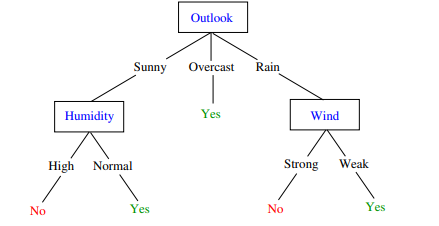
\includegraphics[width=0.6\textwidth]{dtree.png}
    \end{center}
    where:
    \begin{itemize}
        \item $Outlook\in\{Sunny, Overcast, Rain\}$
        \item $Humidity\in\{High, Normal\}$
        \item $Wind\in\{Weak, Strong\}$
        \item $PlayTennis?\in\{Yes, No\}$
    \end{itemize}

    Every node tests an attribute. Each branch corresponds to one of the possible values for that attribute. Each leaf node assigns a classification (Yes or No), in other words predicts the answer $Y$.

    The prblem configurationg is the following:
    \begin{itemize}
        \item $X$ is the set of all possible $x\in X$ that corresponds to a vector of attributes $(Outlook, Humidity, Wind, Temp)$ 
        \item Target function $f:X\to Y$ is the function that maps the attributes to the target variable $PlayTennis?$ (booleans)
        \item Hypothesis space $H=\{h | h:X\to Y\}$ is the set of all possible decision trees that can be constructed using the attributes in $X$ to predict the target variable $Y$
    \end{itemize}

    \begin{center}
        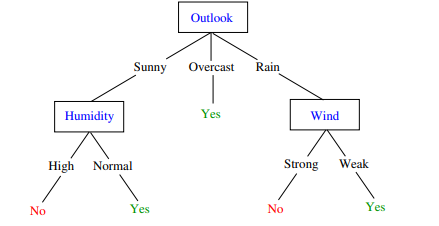
\includegraphics[width=0.6\textwidth]{dtree.png}
    \end{center}
}

\subsection{Top-down inductive construction}
Let $X = X_1 \times X_2 \dots \times X_n $ where $X_i = \{\text{Truee},\text{False}\}$


Can we represent, for instance, $ Y = X_2 \land X_5$? or $Y=X_2 \land X_5 \lor (\lnot X_3) \land X_4 \land X_1 ? $

and:

\begin{itemize}
    \item do we have a decision tree for each h in the space hypothesis?
    \item if the tree exists, is it unique?
    \item if it is not unique, do we have a preference?
\end{itemize}

\thm{
    Basta - Bonzo
}{
    Main loop:
    \begin{itemize}
        \item \textbf{Pick the "best" attribute $X_i$}: At the current node, choose which featue/attribute will bwst split the training data.
        
        Best means: the attribute that gives the most information gain
        \item \textbf{Create a child node for each possible value of $X_i$}: for instance if attribute is "weather" with values "sunny", "rainy", "overcast", create three child nodes.
        \item \textbf{check if all examples in the chils node are pure}: if all examples belong to the same class (e.g., all "yes" or all "no"), make that node a leaf node with that class label. If not repeat the process recursively for each child node.
    \end{itemize}
}

\subsection{Entropy}

\dfn{
    Entropy
}{
    The entropy $H(S)$ of a set of examples $S$ is defined as:
    \[
        H(S) = -\sum_{i=1}^{n} P(X=i)\log_2 P(X=i)
    \]
    where:
    \begin{itemize}
        \item $P(X=i)$ is the proportion of examples in $S$ that belong to class $i$
        \item $n$ is the number of classes (the number of possibile values of $X$)
    \end{itemize}
}

In other words, Entropy meausers the \textit{degree of uncertainty} of the information. It is maximal when $X$ is uniformly distributed (all classes have the same probability) and minimal (zero) when all examples belong to the same class (pure set)
\begin{center}
    \IfFileExists{imgs/entropy.png}{%
        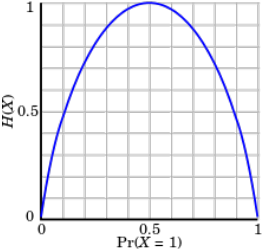
\includegraphics[width=0.6\textwidth]{imgs/entropy.png}%
    }{%
        \fbox{\parbox{0.6\textwidth}{\centering Missing image: imgs/entropy.png}}%
    }
\end{center}

\subsubsection{Information Theory (Shannon 1948)}
The entropy is the average amount of information produced by a stochastic source of data. The \textit{information} is associated to the \textit{probability} of each datum (the surprise element):
\begin{itemize}
    \item An event with probability 1 (certain event) provides no information (no surprise): \(I(1)=0\).
    \item An event with probability 0 (impossible event) provides infinite information (really surprising): \(I(0)=\infty\).
    \item Given two independent events \(A\) and \(B\), the information provided by both events is the sum of the information provided by each event:
    \[
        I(A \cap B) = I(A) + I(B)
    \]
\end{itemize}
So is natoral defining 
\[
    I(p) = -\log_2(p)
\]
\subsubsection{Code Theory (Shannon-Fano 1949, Huffman 1952)}
The entropy is also related to the avarage number of bits required to transmit outcomes produces by a stochastic source process $x$.

Let suppose to have $n$ events with same probability \(p_i = \frac{1}{n}\). Home many bits do we need to encode these events? The answer is \(\log_2(n)\) bits. For instance, if we have 4 events, we need 2 bits to encode them:.

In this case:
\[
    H(X) = -\sum_{i=1}^{n} P(X=i)\log_2 P(X=i) = - \sum_{i=1}^{n} \frac{1}{n} \log_2 \frac{1}{n} = \log_2(n)
\]

\subsection{Information Gain}

In a decision tree, the goal is to maximize the information gain during the execution of the algorithm. 
In other words, the final split should result in the minimum possible impurity. 
Here are the main formulas:

\thm{Entropy of $X$}{
    \[
        H(X) = -\sum_{i=1}^{n} P(X=i)\log_2 P(X=i)
    \]
}

\thm{Conditional Entropy of $X$ given a specific $Y=v$}{
    \label{thm:cexyv}
    \[
        H(X \mid Y=v) = -\sum_{i=1}^{n} P(X=i \mid Y=v)\log_2 P(X=i \mid Y=v)
    \]
}

This measures the entropy of $X$ restricted to the subgroup where $Y=v$.

\thm{Conditional Entropy of $X$ given $Y$}{
    \[
        H(X \mid Y) = \sum_{v=1}^{m} P(Y=v) \, H(X \mid Y=v)
    \]
}

This is the generalization of \ref{thm:cexyv}, used to evaluate the utility of an attribute. 
It measures the average impurity that remains in $X$ after splitting the data using all possible values of $Y$.

\thm{
    Information Gain between $X$ and $Y$
}{
    Here we are!
    \begin{math}
        I(X, Y ) = H(X) - H(X\|Y ) = H(Y ) - H(Y \|X)
    \end{math}
}

\ex{Information gain}{
    Let us measure the entropy reduction of the target variable $Y$ due to some attribute $X$, that is the information gain $I(Y , X)$ between $Y$ and $X$

    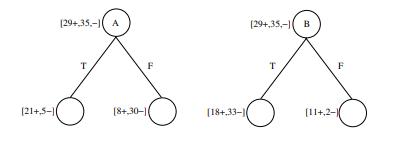
\includegraphics{ig.png}

    \[
    \begin{aligned}
    H(Y) &= -\frac{29}{64}\log_2\!\left(\tfrac{29}{64}\right) - \frac{35}{64}\log_2\!\left(\tfrac{35}{64}\right) = 0.994 \\[6pt]
    H(Y \mid A=T) &= -\frac{21}{26}\log_2\!\left(\tfrac{21}{26}\right) - \frac{5}{26}\log_2\!\left(\tfrac{5}{26}\right) = 0.706 \\[6pt]
    H(Y \mid A=F) &= -\frac{8}{38}\log_2\!\left(\tfrac{8}{38}\right) - \frac{30}{38}\log_2\!\left(\tfrac{30}{38}\right) = 0.742 \\[6pt]
    H(Y \mid A) &= 0.706 \cdot \tfrac{26}{64} \;+\; 0.742 \cdot \tfrac{38}{64} = 0.726 \\[6pt]
    I(Y, A) &= H(Y) - H(Y \mid A) = 0.994 - 0.726 = 0.288 \\[6pt]
    H(Y \mid B) &= 0.872 \\[6pt]
    I(Y, B) &= 0.122
    \end{aligned}
    \]
}

% TODO: LA PARTE DELLA CONITINUITÀ
\chapter{Overfitting}
Let us consider the error of the hypothesis $h$
\begin{itemize}
    \item on the training set, $error_{train}(h)$
    \item on the full data set $\mathcal{D}$, $error_{\mathcal{D}}(h)$ 
\end{itemize}

\dfn{Overfitting}{
    It's said taht $h$ \textit{overfits} the training set if there exixsts another
     hypotheses $h'$ such that:
     \[
        \et{h}<\et{h'}
     \]
     but
    \[
        \ed{h} > \ed{h'}
    \]
}

These models ($h$ and $h'$) represent two different situations.
The first corresponds to a model that fits the training dataset very closely, including its uncertainty and noise.
The second is simpler: it captures only the general trend of the training data and avoids fitting the noise.
As a consequence, the error with respect to the true data distribution $\mathcal{D}$ is larger for the first model than for the second.
The second one is better! Let's generalised.

But \textit{We do not know} $\D$

\section{Avoiding the over fitting}
\subsection{Detecting the Overfitting: validation set}
For Detecting the Overfitting it's usefull divinding the dats aviables in two disjoint sets:
\begin{itemize}
    \item \textbf{Training set}: set of datas that the model \textit{use for learning}. The dtree is built by this datas
    \item \textbf{validation set}: This set is not shown during the training- It's used as "test" for evaluating the accuracy of the model
\end{itemize}

\subsection{Early stopping}
This is a proactive strategy. Instead of let the tree grows untill his major complexity, it's sopped first the possibility of Overfitting. The growing of a branch is stopped if these two conditions is verified:
\begin{itemize}
    \item \textbf{The improvement is too small}: if a possible divsion of datas produces a gain of information below a certain threshold, it means that it's not usefull to continue
    \item \textbf{There are not enaugh datas}: if a node contains a number of examples too musch low, any decision taken would be statistically unreliable and probably based on noise. The tree stops to avoid creating rules based on coincidences.
\end{itemize}
\subsection{Post - Pruning}
This strategy is \textbf{reactive}. 
The decision tree is let grow completely on the training set, 
which may lead to overfitting, 
and then the useless or harmful branches are pruned.

\dfn{Reduce-Error Post-Pruning}{
    The \textit{reduce-error post-pruning} technique works as follows:
    \begin{itemize}
        \item build the tree completely
        \item evaluate each branch using a validation set
        \item prune the branch whose removal improves accuracy the most
        \item repeat until no further pruning improves the accuracy
    \end{itemize}
}



% \begin{document}
\newcounter{assiomacounter} 
\newcommand{\assiomalabel}[1]{\refstepcounter{assiomacounter}\label{#1}\textbf{Assioma \theassiomacounter.}}

\chapter{Spazi di probabilità}
\section{Concetti introduttivi}
Innanzi tutto andiamo a definire che cosa intendiamo per \textit{esperimento aleatorio, esito, probabilità}

Con la dicitura \textit{esperimento aleatorio} indicheremo qualunque fenomeno (fisico, economico, sociale, \dots ) il cui esito non sia determinabile con certezza a priori. Il nostro obiettivo è di fornire una descrizione matematica di un esperimento aleatorio, definendo un modello probabilistico, un \textit{esito} invece è un ipotetico risultato di un'esperimento aleatorio sulla base di un cosiddetto \textit{spazio campionario} un insieme che contiene tutti gli esiti possibili dell’esperimento

\esempio{
    \begin{itemize}
        \item \textbf{Esperimento aleatorio:} Lancio di un dado.
        \item \textbf{Spazio campionario:} $\Omega = \{1, 2, 3, 4, 5, 6\}$.
        \item \textbf{Esito:} $4$.
    \end{itemize}
}

\nt{
  In casi piu' complessi ci saranno vari sotto-esperimenti aleatori, come 10 lanci di un dato.
}

Adesso forniamo vere e priorie definizioni
\dfn{evento}{
    Si definisce \textbf{evento} un'affermazione riguardante l'ipotetico esito univoco dell'esperimento, di cui si può affermare con certezza se è vero o falso una volta noto l'esito
}
\ex{}{
    Esper. aleatorio: Lancio del dado\\
    $A = \text{"esce un numero pari"}$
}

\dfn{Spazio camipionario}{
  Lo \textbf{spazio campionario} è l'insieme di tutti i possibili esiti di un esperimento casuale e viene denotato con $\Omega$
}

Notare che non si afferma "tutti e solo tutti", quindi \textbf{qualsiasi} insieme che contiene gli esiti possibili può essere considerato uno spazio campionario

\ex{Lancio dado}{
  Possiamo porre come spazio campionario:
  \[
  \Omega = \{1,2,3,4,5,6\}
  \]
  ma anche
  \[
  \Omega = \mathbb{R}
  \]
}

\dfn{Esiti favorevoli}{
  Esiti per cui un evento è vero sono detti esiti favorevoli.
}

\dfn{Evento in termine di insiemi}{
  Un evento si puo' definire anche come il sottoinsieme dello spazio campionario $ \Omega $ formato da tutti gli esiti favorevoli dell'evento.
}

\ex{}{
$ \Omega = \{1,2,3,4,5,6\} \implies A = \text{"esce un numero pari"} \implies \{2,4,6\} $ sono gli esiti favorevoli dell'evento $A$.
 } 

 \nt{
  La definizione insiemistica di un evento dipende dallo spazio campionario $\Omega$ definito, poiché l'evento è un sottoinsieme di $\Omega$. Tuttavia, l'insieme degli esiti favorevoli di un evento è fisso, e rappresenta l'insieme evento di cardinalità massima possibile, ovvero l'insieme degli esiti favorevoli $A \subseteq \Omega$.
  }

\dfn{}{
  \begin{itemize}
    \item $ \Omega $ e' l'evento \textit{certo}
    \item $ \emptyset $ e' l'evento \textit{impossibile}
    \item $ \omega \in \Omega $ e' un evento \textit{elementare} ($ A = \{\omega\} $)
  \end{itemize}
}
\ex{}{
Lancio un dado.
\[
A = \text{"esce un numero tra 1 e 6"}
\]
\[
B = \text{"esce un numero maggiore di 6"}
\]
\[
C = \text{"esce il numero 3"}
\]
\begin{itemize}
    \item Se $\Omega = \{1,2,3,4,5,6\}$, allora:
    \begin{itemize}
        \item $A = \Omega$ (evento certo), 
        \item $B = \emptyset$ (evento impossibile), 
        \item $C = \{3\}$ (evento con un solo esito favorevole).
    \end{itemize}
    \item Se $\Omega = \mathbb{R}$, allora:
    \begin{itemize}
        \item $A = \{1,2,3,4,5,6\} \subset \Omega$ (evento quasi certo),
        \item $B = (6,+\infty)$ (evento quasi impossibile),
        \item $C = \{3\}$ (evento con un solo esito favorevole).
    \end{itemize}
\end{itemize}
}


\section{Regole del calcolo probabilistico}
Ad ogni relazione logica possiamo associare un'operazione insiemistica:

\begin{center}
  \begin{tabular}{c|c}
    Connettivi Logici & Connettvi Insiemistici\\
    \hline
    $ A \lor B $ & $ A \cup B $ \\
    $ A \land B $ & $ A \cap B $ \\
    $ \neg A $ & $ A^{c} $ \\
    $ A \implies B $ & $ A \subseteq B $ \\
    $ A \iff B $ & $ A = B $
\end{tabular}
\end{center}

\nt{
  Nella prima colonna, $ A $ e $ B $ sono eventi come affermazioni, mentre nella colonna di destra sono degli insiemi.
}


\subsection{Assiomi della probabilita'}
Poniamo tre assiomi fondamentali da cui possiamo partire per derivare tutte le operazioni e proprieta' che ci servono:

\nt{
  Per noi tutti i sottoinsiemi di $ \Omega $ sono eventi (anche se non sara' sempre cosi)
}

\dfn{Assiomi fondamentali della probabilità}{
  \assiomalabel{assioma1} A ciascun sottoinsieme (o evento) $A$ di $\Omega$ è assegnato un numero $\mathbb{P}(A)$ che verifica:
  \[ 0 \leq \mathbb{P}(A) \leq 1. \]
  Tale numero $\mathbb{P}(A)$ si chiama \textbf{probabilità} dell'evento $A$.

  \assiomalabel{assioma2} $\mathbb{P}(\Omega) = 1$.

  \assiomalabel{assioma3} Vale la proprietà di \textbf{additività numerabile}\footnote{Anche detta \textbf{$\sigma$-additività}.}: sia $A_1, A_2, \ldots, A_n, \ldots$ una successione di sottoinsiemi di $\Omega$ tra loro disgiunti\footnote{In formule: $A_i \cap A_j = \emptyset$, per ogni $i \neq j$. In altri termini, non hanno elementi in comune.} e sia
  \[ A = \bigcup_{n=1}^{\infty} A_n. \]
  Allora
  \[ \mathbb{P}(A) = \sum_{n=1}^{\infty} \mathbb{P}(A_n). \]
}

\nt{
  Quindi, per il primo assioma, esiste una funzione probabilita' $ \mathbb{P}(A): \powerset (\Omega) \to [0,1] $.
}

\dfn{Spazio di probabilità}{
La coppia $(\Omega, \mathbb{P})$ si dice \textbf{spazio di probabilità} o modello matematico dell’esperimento aleatorio
}

\subsection{Conseguenze degli assiomi}

\thm{}{
  Sia \( \Omega \) spazio campionario e \( \mathbb{P} \) probabilità su \( \Omega \) (\( (\Omega, \mathbb{P}) \) è uno spazio di probabilità con \( \mathbb{P}: \powerset(A) \to [0,1] \)). Dagli assiomi \ref{assioma1}, \ref{assioma2}, \ref{assioma3} deduciamo le cose seguenti:
  \begin{enumerate}
  \item \( \mathbb{P}(\emptyset) = 0 \)
  \item \label{item:finite_additivity} \textbf{Additività finita}: \( (A_i)_{i = 1,\ldots,n}.\ \forall i \neq j.\, A_i \cap A_j = \emptyset \implies \mathbb{P}\left(\bigcup_{i=1}^{n} A_i\right) = \sum_{i=1}^{n} \mathbb{P}(A_i) \)
  \item \( \mathbb{P}(A^c) = 1 - \mathbb{P}(A) \)
  \item \textbf{Monotonia}: \( A \subseteq B \implies \mathbb{P}(A) \leq \mathbb{P}(B) \)
  \end{enumerate}
}

\pf{Dimostrazione}{

  \begin{enumerate}
    \item Devo mostrare che \( \mathbb{P}(\emptyset) = 0 \). Per semplicità definiamo \( p \coloneqq \mathbb{P}(\emptyset) \). Uso l'assioma \ref{assioma3} con la successione \( (A_n)_{n \in \mathbb{N}} \) dove \( \forall i \in \mathbb{N}.\, A_i = \emptyset \), che sono tutti eventi disgiunti. Quindi:
    \[
      \mathbb{P}\left(\bigcup_{i=1}^{\infty} A_i\right) = \sum_{i=1}^{\infty} \mathbb{P}(A_i) = \sum_{i=1}^{\infty} p.
    \]
    Inoltre:
    \[
      \bigcup_{i=1}^{\infty} A_i = \emptyset \implies p = \sum_{i=1}^{\infty} p.
    \]
    L'equazione è soddisfatta solo per \( p = 0 \).

    \item Supponiamo di avere una sequenza finita disgiunta \( A_1, \ldots, A_n \). Definisco \( (B_i)_{i \in \mathbb{N}} \) tale che \( B_i = A_i \) per \( i = 1,\ldots,n \) e \( B_i = \emptyset \) per \( i > n \). Usando l'assioma \ref{assioma3}:
    \[
      \mathbb{P}\left(\bigcup_{i=1}^{\infty} B_i\right) = \sum_{i=1}^{\infty} \mathbb{P}(B_i) = \sum_{i=1}^{n} \mathbb{P}(A_i).
    \]

    \item Per definizione di complemento, \( A^c \cup A = \Omega \) e \( A^c \cap A = \emptyset \). Per additività:
    \[
      \mathbb{P}(A^c) + \mathbb{P}(A) = \mathbb{P}(\Omega) = 1 \quad (\text{per l'assioma \ref{assioma2}}).
    \]

    \item Se \( A \subseteq B \), allora \( B = A \cup (B \setminus A) \), con \( A \) e \( B \setminus A \) disgiunti. Per additività:
    \[
      \mathbb{P}(B) = \mathbb{P}(A) + \mathbb{P}(B \setminus A) \geq \mathbb{P}(A).
    \]
  \end{enumerate}
}

\thm{Probabilità unione non disgiunta}{
  Siano \( A \) e \( B \) eventi:
  \begin{equation}
    \label{eq:unione}
    \mathbb{P}(A \cup B) = \mathbb{P}(A) + \mathbb{P}(B) - \mathbb{P}(A \cap B)
  \end{equation}
    
  
}

\pf{Dimostrazione}{
  \( A \cup B = (A \setminus B) \cup (B \setminus A) \cup (A \cap B) \). Per additività:
  \[
    \mathbb{P}(A \cup B) = \mathbb{P}(A \setminus B) + \mathbb{P}(B \setminus A) + \mathbb{P}(A \cap B).
  \]
  Osservando che:
  \[
    \mathbb{P}(A \setminus B) + \mathbb{P}(A \cap B) = \mathbb{P}(A), \quad \mathbb{P}(B \setminus A) + \mathbb{P}(A \cap B) = \mathbb{P}(B),
  \]
  si ottiene la formula.
}

\nt{
  La formula si complica con un numero di eventi maggiore di 2. Per \( n=3 \):
  \[
    \mathbb{P}(A \cup B \cup C) = \mathbb{P}(A) + \mathbb{P}(B) + \mathbb{P}(C) - \mathbb{P}(A \cap B) - \mathbb{P}(B \cap C) - \mathbb{P}(A \cap C) + \mathbb{P}(A \cap B \cap C).
  \]
}
\section{Probabilita' discreta} \label{dfn:probDiscr}
Finora sappiamo solo le "regole" che deve seguire una funzione per essere una probabilita'. Passiamo ora a vedere come calcolare il valore di un certo tipo di probabilita', la \textit{probabilita' discreta}:
\dfn{Probabilità discreta}{
  Chiamo probabilità discreta una funzione probabilità \( \mathbb{P} \) su $ \Omega $, tale che:
  \[
    \exists \overline{\Omega} \subseteq \Omega,\ \overline{\Omega} \text{ e' finito o numerabile}.\ \mathbb{P}(\overline{\Omega}) = 1
  \]
}

Ovvero, una probabilita' e' discreta se il suo spazio campionario minimo e' finito o numerabile. Questa condizione e' necessaria per poter poi definire un modo per effettivamente calcolare il valore della probabilita' (discreta) di un qualunque evento.

Diamo prima una definizione di una tale probabilità:
\dfn{Delta di Dirac}{
  Sia \( \Omega = \mathbb{R} \), \( x_0 \in \mathbb{R} \), allora si chiama delta di Dirac centrato in \( x_0 \) la funzione:
\[
  \begin{aligned} 
    \delta_{x_0}: \powerset(\mathbb{R}) &\to [0,1]\\
    A &\mapsto \delta_{x_0}(A) = \begin{cases}
    1 & x_0 \in A\\
    0 & x_0 \notin A
    \end{cases}
  \end{aligned}
\]
}

Notare che per definizione, la funzione di Dirac è una probabilità discreta, dato che soddisfa tutti gli assiomi per essere una probabilita' e il suo spazio campionario minimo e' formato da un solo elemento di $ \Omega $, quindi e' discreta (ma non molto utile dato che puo' assumere solo due valori). Però, tramite le delta di Dirac, siamo in grado di costruire qualunque altra probabilità discreta:

Sia \( \Omega = \mathbb{R} \). Prendiamo un numero contabile \( n \) di eventi singoletto \( x_1,x_2,\ldots,x_n \in \mathbb{R} \) a cui corrispondono \( p_1,p_2,\ldots,p_n \in \mathbb{R} \) tale che:
\[
 \forall i = 1,\ldots,n.\ p_i \in [0,1], \qquad  \sum_{i=1}^{n} p_i = 1 
\]
Definiamo la funzione:
\[
\begin{aligned}
  \mathbb{P}: \powerset(\Omega) &\to [0,1]\\
  A &\mapsto \sum_{i=1}^{n} p_i \delta_{x_i}(A)
\end{aligned}
\]
\( \mathbb{P} \) è una combinazione lineare di delta di Dirac. Essendo una combinazione convessa, \( \mathbb{P} \in [0,1] \) e si può dimostrare che soddisfa gli altri due assiomi (\ref{assioma2} e \ref{assioma3}), quindi è una probabilità discreta! Variando le \( x \) e le \( p \) è possibile generare qualsiasi funzione \( \mathbb{P} \) discreta.

\ex{}{
  \( \Omega = \{1,2,3,4,5,6\},\ \forall i = 1,\ldots,6.\ x_i = i,\ p_i = \frac{1}{6} \), la funzione \( \mathbb{P} \) associata è:
  \[
   P(A) = \sum_{ i=1}^{6} \frac{1}{6} d_{x_i}(A)
  \]
  \[
    A = \{1,2,3,4,5,6\} \implies P(A) = 1 
  \]
  \[
    B = (6,+\infty) \implies P(B) = 0
  \]
  \[
    C = \{1,2,3,4,5,6,7,8,9\} \implies P(C) = 1
  \]
}

\dfn{}{
  Si chiama evento quasi certo un evento \( A \) tale che \( \mathbb{P}(A) = 1 \).
}

\dfn{}{
  Si chiama evento quasi impossibile un evento \( A \) tale che \( \mathbb{P}(A) = 0 \).
}

Posso allargare \( \Omega \) quanto voglio perché tanto fuori dall'insieme minimo che comprende tutti gli eventi possibili le probabilità che aggiungo sono quasi impossibili e quindi hanno probabilità 0 e non cambiano il valore totale della somma.

\subsection{Probabilita' uniforme}
\thm{Principio di porbabililità uniforme}{
  Si cosideri un esperimento aleatorio aleatorio con spazio campionario \( \Omega = \{w_1,\dots, w_N\} \) finito e discreto, con esiti sono equiprobabili $\mathbb{P}(\{w_1\}) = \mathbb{P}(\{w_2\}) =\dots = \mathbb{P}(\{w_N\})$.

  Si dice allora che $\mathbb{P}$ è la \textbf{probabilità uniforme} su $\Omega$ e valgono le seguenti proprietà:
  \begin{enumerate}
    \item Dato un qualunque evento elementare $A = \{w_i\}$, si ha:
    \[
      \mathbb{P}(A) = \frac{1}{N}
    \]
    \item Dato un qualunque evento $A \subseteq \Omega$, vale la \textit{formula di Laplace}:
    \[
      \mathbb{P}(A) = \frac{|A|}{N} = \frac{\text{numero di esiti favorevoli}}{\text{numero di esiti possibili}}
    \]
  \end{enumerate}
}

\pf{Dimostrazione}{
  \begin{enumerate}
    \item Dimostro il punto 1:
    
    Per ipotesi sappiamo che $\mathbb{P}(\{w_1\}) = \mathbb{P}(\{w_2\}) =\dots = \mathbb{P}(\{w_N\})$ e per il \textit{principio di additività} si può costruire il seguente sistema:
    \[
      \begin{cases}
        \mathbb{P}(\{w_1\}) + \mathbb{P}(\{w_2\}) + \dots + \mathbb{P}(\{w_N\}) = 1\\
        \mathbb{P}(\{w_1\}) = \mathbb{P}(\{w_2\}) \\
        \mathbb{P}(\{w_2\}) = \mathbb{P}(\{w_3\}) \\
        \vdots\\
        \mathbb{P}(\{w_{N_1}\}) = \mathbb{P}(\{w_N\})
      \end{cases}
    \]
    Da cui si ricava che: 
    \[\forall i\in[1,\dots, N] \quad \mathbb{P}(\{w_i\}) = \frac{1}{N}\]

    \item Dimostro il punto 2:
    Sia $A = \{w_{i_1},\dots,w_{i_k}\}$, con $k \leq N$. Per definizione di probabilità:
    \[
      \mathbb{P}(A) = \mathbb{P}(\{w_{i_1},\dots,w_{i_k}\}) = \mathbb{P}(\{w_{i_1}\}) + \dots + \mathbb{P}(\{w_{i_k}\}) = \frac{k}{N}
    \]
  \end{enumerate}
}
% \end{document}

% \begin{document}
\chapter{Probabilita' Condizionata}

\section{Definizione e motivazioni}

Supponiamo di sapere che un evento di un'esperimento aleatorio si e' avverato. Finora abbiamo visto solo casi in cui gli eventi non si influenzavano (\textit{indipendenti}), ma succede spesso nella realta' che se si sa che un certo evento e' avvenuto, allora questo ci da' informazioni aggiuntive che possono cambiare la probabilita' di altri eventi di cui ancora non sappiamo gli esiti.

Chiamiamo $ B $ l'evento che e' avvenuto e $ A $ un altro evento di cui vogliamo sapere la probabilita'. Prima di avere informazioni su $ B $, la probabilita' di $ A $ era semplicemente $ \mathbb{P}(A) $, ma ora ci poniamo la domanda: "se so che si e' verificato $ B $, come cambia $ \mathbb{P}(A) $?". Denotiamo questa nuova probabilita' con:
\[
  P(A|B)
\]
chiamata la \textit{probabilita' condizionata di  A  dato  B }.

\dfn{Probabilita' Condizionata}{
  Prendo due eventi $ A, B $ su uno spazio di probabilita' $ \left( \Omega, \mathbb{P} \right) $. Definisco \textit{probabilita' condizionata a B di A} la funzione:
  \begin{align*}
    \mathbb{P}(A|B): \powerset(\Omega) &\to [0,1]\\
    A &\mapsto \frac{\mathbb{P}(A \cap B)}{\mathbb{P}(B)}
  \end{align*}
}
E' possibile dimostrare che una certa funzione e' anch'essa una probabilita' (sempre discreta), verifichiamo gli assiomi (fissiamo $ B \subseteq \Omega $ con $ \mathbb{P}(B) > 0 $):
\begin{enumerate}
  \item $ \mathbb{P}(A|B) \in [0,1], \forall A \subseteq \Omega $
  \item $ \mathbb{P}(\Omega|B) = 1 $
  \item $ \sigma-\text{addittivita'} $: $ (A_i)_{i \in \mathbb{N}} $ disgiunti:
    \[
      \mathbb{P}(\bigcup_{i=1}^{\infty} A_i|B) = \sum_{i=1}^{\infty} \mathbb{P}(A_i|B)
    \]
\end{enumerate}
Lasciate al lettore in quanto davvero molto facili, quasi banali. Se non riesci a farle fai schifo.

Vediamo ora, con un esempio, come mai e' proprio questa la definizione utilizzata:
\ex{}{
  \begin{itemize}
  \item 
  Lancio del dado: $ \Omega = \{1,2,3,4,5,6\} $, $ \mathbb{P} $ probabilita' uniforme:

  $ \mathbb{P}(\{\omega\}) = \frac{1}{|\Omega|}, \forall \omega \in \Omega $, ovvero:
  \[
    \mathbb{P}(A) = \frac{\text{casi favorevoli in }A}{\text{casi possibili}}
  \]
  $ A = \text{"esce un numero maggiore di 3"} = \{3,4,5,6\} $ e $ B = \{\text{"esce un numero pari"}\} = \{2,4,6\} $, domanda: quanto vale $ \mathbb{P}(A|B) $?

  $ P(A) = \frac{4}{6} $ come abbiamo gia visto.

  Ora abbiamo un'informazione in piu': sappiamo che $ B $ si e' avverato. Questo significa che si restringe l'insieme di valori che possono essere usciti al lancio del dado. ATTENZIONE! cio' non vuol dire che cambia lo spazio campionario perche' l'esperimento e' lo stesso, ma cambiano i \textit{veri} casi favorevoli e i \textit{veri} casi possibili:
  \[
    P(A|B) = \frac{\text{"veri casi favorevoli di A"}}{\text{veri casi possibili}} = \frac{|A \cap B|}{|B|} = \frac{2}{3}
  \]
  \item
  Vediamo anche cosa accade quando la probabilita' non e' uniforme, come con un dado a 4 facce truccato: 

  $ \Omega = \{1,2,3,4\} $, $ \mathbb{P}(4)=\frac{1}{15}, \mathbb{P}(3)=\frac{2}{15}, \mathbb{P}(2)=\frac{4}{15}, \mathbb{P}(1)=\frac{8}{15} $

  $ A = \{3,4\}, B = \{2,4\} $
  \[
    \mathbb{P}(A|B) = \frac{\text{"probabilita' dei veri casi favorevoli di A"}}{\text{probabilita' dei veri casi possibili}} = \frac{\mathbb{P}(A \cap B)}{\mathbb{P}(B)}
  \]
  \end{itemize}

}

\nt{
  Se $ \mathbb{P} $ e' la probabilita' uniforme allora:
  \[
    \mathbb{P}(A|B) = \frac{\mathbb{P}(A \cap B)}{\mathbb{P}(B)} = \frac{\frac{|A \cap B|}{|\Omega|}}{\frac{|B|}{|\Omega|}} = \frac{|A \cap B|}{|B|}
  \]
}

\nt{
  B e' fissato nella definizione di propbabilita' condizionata, ovvero:
  \[
    \mathbb{P}(A|B) \neq \mathbb{P}(B|A)
  \]
  Quindi il ruolo di $ A $ e $ B $ e' completamente diverso
}

\nt{
  Se $ B = \Omega $, allora $ \mathbb{P}(A|B) = \mathbb{P}(A) $ dato che la conoscenza del fatto che si e' avverato $ \Omega $ e' ovvio e non ci cambia.

  Se $ A = \Omega $, allora $ \mathbb{P}(\Omega | B) = 1 $ (per proprieta', dato che e' sempre una probabilita')
}

\section{Regola della catena}

La probabilita' condizionata in genere e' nota e si usa per calcolare la probabilita' dell'intersezione:
  \[
    \mathbb{P}(A \cap B) = \mathbb{P}(A|B) \cdot \mathbb{P}(B)
  \]
Questa formula e' detta \textit{regola della catena} e vale in generale con $ n $ eventi:

\mprop{Regola della catena (generalizzata)}{
  $ (A_i)_{i = 1,...,n}, \mathbb{P}(A_1 \cap ... \cap A_{n-1}) > 0 $, allora:
  \[
    \mathbb{P}(A_1 \cap ... \cap A_n) = \mathbb{P}(A_1)\mathbb{P}(A_2|A_1)\mathbb{P}(A_3|A_1 \cap A_2) ... \mathbb{P}(A_n| A_1 \cap ... A_{n-1})
  \]
}
\nt{

  La condizione funziona grazie alla monotonia, dato che $ 0 < \mathbb{P}(A_1 \cap ... \cap A_{n-1}) \leq \mathbb{P}(A_1 \cap ... \cap A_j), 1 \leq j \leq n-1 $ quindi siamo certi che l'intersezione degli eventi che sono avvenuti e' maggiore di 0.
}
\pf{}{
  $ P(A_1) \frac{P(A_1 \cap A_2)}{P(A_1)}...\frac{P(A_1 \cap ... \cap A_n)}{P(A_1 \cap ... \cap A_{n-1})}= P(A_1 \cap ... \cap A_n) $
} 
TODO: migliora un po

\ex{}{
Un’urna contiene tre palline bianche, due palline nere e una pallina rossa.
Si eseguono tre estrazioni senza reimmissione.
Qual `e la probabilit`a di estrarre nell’ordine una bianca, una rossa e una nera?

  Sono interessato solo ad alcuni eventi, quindi non c'e' bisogno di descrivere l'intero esperimento aleatorio. Per prima cosa definisco l'evento:
  \[
  A = \text{"estrarre in ordine una bianca, una rossa e una nera"}
  \]
  Voglio trovare $ P(A) $. Notiamo che dobbiamo determinare tre sottoesperimenti in relazione (dato che non c'e' reimissione). Quindi dopo ogni sottoesperimento cambia la composizione dell'urna, e sappiamo come calcolare la probabilita' condizionata:
  \[
  B_i = \text{"estraggo una pallina bianca all' i-esimo turno"}
  \]
  \[
  R_i = \text{"estraggo una pallina rossa all' i-esimo turno"}
  \]
  \[
  N_i = \text{"estraggo una pallina nera all' i-esimo turno"}
  \]
  Esistono tre famiglie di eventi: $ (B_i)_{i = 1,...,k}, (R_i)_{i = 1,...,k}, (N_i)_{i = 1,...,k} $ dove $ i $ indica il turno al quale viene estratta la pallina. Quindi possiamo scrivere $ A $ come relazione fra sottoeventi:
  \[
  A = B_1 \cap R_2 N_3
  \]
  Quindi:
  \[
    P(A) = P(B_1 \cap R_2 \cap N_3) = P(B_1)P(R_2 | B_1)P(N_3 | B_1 \cap R_2)
  \]
  Solo ora possiamo passare ai valori numerici. Dato che gli esiti sono equiprobabili e lo spazio campionario e' finito, la probabilita' e' uniforme:
  \[
    P(B_1) = \frac{1}{2}, P(R_2) = \frac{1}{5}, P(N_3) = \frac{1}{2}
  \]
  \[
    P(A) = \frac{1}{20}
  \]
}

Per esperimenti formati da sottoesperimenti di cui conosco le probabilita' condizionate, e' possible rappresentare ogni evento come un nodo:
\[
\Omega = \text{primo nodo}
\]
e ogni probabilita' come un ramo che partiziona il nodo (tanti rami quanti gli insiemi della partizione) che rappresenta poi un altro evento (condizionato dalla seconda in poi).

\begin{center}
  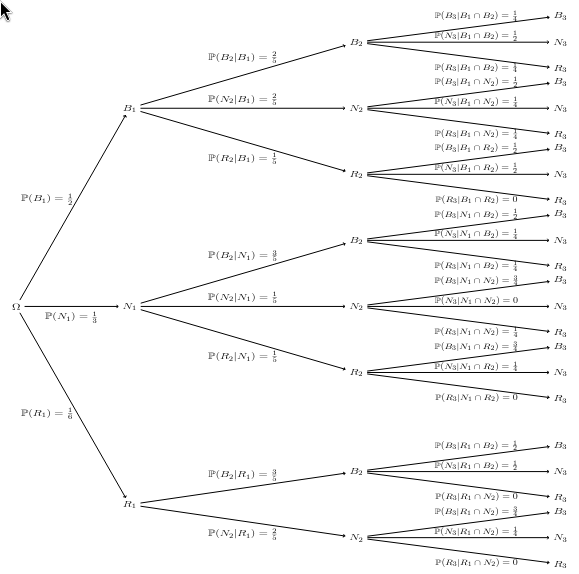
\includegraphics[width=0.5\textwidth]{img/2025-02-28-13-59-32.png}
\end{center}

La regola della catena la leggo sul diagramma ad albero:

percorso: $ \Omega \to B_1 \to R_2 \to N_3 $ ha probabilita' $ P(B_1 \cap R_2 \cap N_3) $ che si calcola facendo il prodotto delle probabilita' dei relativi rami che si usano nel percorso.

E' uno strumento utile per convincerci che stiamo usando le formule guiste, ma non le sostituisce e puo' diventare laborioso per problemi complessi.

\ex{}{
Ci sono due urne: la prima contiene due palline rosse e una bianca; la
seconda contiene tre palline rosse e due bianche. Si lancia una moneta: se esce testa si
estrae una pallina dalla prima urna, se esce croce si estrae una pallina dalla seconda urna.
Qual `e la probabilit`a che l’esito del lancio della moneta sia testa e la pallina estratta sia
bianca?

  2 sottoesperimenti:
  \begin{itemize}
  \item lancio della moneta
  \item estrazione da un'urna
  \end{itemize}

  Nota che i sottoesperimenti sono indipendenti dall'esito di altri esperimenti. Sono gli esiti, ovvero i risultati, che possono dipendere dagli esiti di altri esperimenti.

  \[
  A = \text{"esce testa ed estraggo una pallina bianca"}
  \]
  Devo esprimere A con eventi che 
  \[
  T = \text{"esce testa"}
  \]
  \[
  U = \text{estraggo una pallina bianca}
  \]
  Disegna lo zio pera di diagramma che non mi metto a fare, se @GiovanniPalma vuole puo' farlo
  \[
    A = T \cap U, \quad P(A) = P(T)P(U|T)
  \]
}

\section{Indipendenza di eventi}

E' possibile che sapere che un evento $ B $ e' avvenuto non altera la probabilita' di un altro evento $ A $. Possiamo esprimere questa relazione in modo matematico cosi':
\[
  \mathbb{P}(A|B) = \mathbb{P}(A)
\]
Utilizzando la definizione di probabilita' condizionata, possiamo usare un'identita' equivalente che useremo come definizione:
\dfn{Eventi indipendenti}{
  Due eventi $ A, B $ si dicono indipendenti se:
  \begin{equation}
    \mathbb{P}(A \cap B) = \mathbb{P}(A) \cdot \mathbb{P}(B)
  \end{equation}
  

  E viene denatato $A \dperp B$
}

Usiamo questa definizione dato che e' esplicitamente simmetrica, ovvero se A e indipendente a B allora vale anche il contrario:
\[
A \dperp B \iff B \dperp A
\]
ed e' definita (e banalmente vera) anche quando $ \mathbb{P}(A)=0 $ o $ \mathbb{P}(B)=0 $. In particolare si noti il seguente teorema:
\thm{Teorema della simmetria tra eventi indipendenti}{ \label{thm:simmetria_indipendenza}
  Sia $\mathbb{P}(B)>0$ allora:
  \[
    A \dperp B \iff \mathbb{P}(A|B) = \mathbb{P}(A)
  \]
  Dall'altro lato, sia $\mathbb{P}(A)>0$ allora:
  \[
    A \dperp B \iff \mathbb{P}(B|A) = \mathbb{P}(B)
  \]
}

\pf{Dimostrazione}{
  Verrà fornita solo la dimostrazione del primo punto, la seconda parte è analoga.

  Assumo $\mathbb{P}(B)>0$, si ha:
  \begin{itemize}
    \item $ A \dperp B \implies \mathbb{P}(A|B) = \mathbb{P}(A) $:
      \[
        \mathbb{P}(A|B) = \frac{\mathbb{P}(A \cap B)}{\mathbb{P}(B)} = \frac{\mathbb{P}(A) \cdot \mathbb{P}(B)}{\mathbb{P}(B)} = \mathbb{P}(A)
      \]
    \item $ \mathbb{P}(A|B) = \mathbb{P}(A) \implies A \dperp B $:
      \[
        \mathbb{P}(A \cap B) = \mathbb{P}(A|B) \cdot \mathbb{P}(B) = \mathbb{P}(A) \cdot \mathbb{P}(B)
      \]
  \end{itemize}
}

\nt{
  Si noti che se $\mathbb{P}(A)>0$ e $\mathbb{P}(B)>0$ allora, le tre uguaglianze seguenti sono equivalenti:
  \[
    \mathbb{P}(A\cap B) = \mathbb{P}(A) \cdot \mathbb{P}(B) \iff \mathbb{P}(A|B) = \mathbb{P}(A) \iff \mathbb{P}(B|A) = \mathbb{P}(B)
  \]
}

\nt{
  \begin{itemize}
  \item L'indipendenza e' diversa dalla disgiunzione:
  \[
  A \indip B \neq A \cap B = \emptyset
  \]
  infatti sono relazioni ortogonali:
  \[
    A \indip B \land A \cap B = \emptyset \iff \mathbb{P}(A)\mathbb{P}(B) = 0 \iff \mathbb{P}(A) = 0 \lor \mathbb{P}(B) = 0
  \]
  \item L'indipendenza e' diverso dall'essere sottoinsieme non-vuoto:
    \[
    A \indip B \neq A \subseteq B \lor B \subseteq A
    \]
    infatti:
    \[
      A \indip B \land A \subseteq B \iff \mathbb{P}(A)\mathbb{P}(B) = \mathbb{P}(A) \iff \mathbb{P}(B) = 1 
    \]
  \end{itemize}
  
  Quindi in generale due eventi sono indipendent quando la loro intersezione ha "le giuste proporzioni".
}

Adesso fornirò un altro teorema piuttosto importante:
\mprop{Sull'indipendenza di eventi complomentari}{
  Siano $A, B$ due eventi indipendenti, allora:
  \[
    A \dperp B \iff A^c  \dperp B,\, A \dperp B^c,\, A^c \dperp B^c
  \]
}
\pf{Dimostrazione}{
  Dimostro solo la prima parte, le altre sono analoghe.

  Assumo $A, B$ due eventi indipendenti, debbo dimostrare la seguente uguaglianza:
  \[
    \mathbb{P}(A^c \cap B) = \mathbb{P}(A^c) \cdot \mathbb{P}(B)
  \]

  Dato che 
  \[
    B = \Omega \cap B = (A \cup A^c) \cap B = (A \cap B) \cup (A^c \cap B)
  \]

  E dato che $ (A \cap B) $e$ (A^c \cap B)$ sono disgiunti, per \ref{item:finite_additivity} (\textit{additività finita}) si ha:
  \[
    \mathbb{P}(B) = \mathbb{P}(A \cap B) + \mathbb{P}(A^c \cap B)
  \]

  E dato che $ A \dperp B $ si ha:
  \[
    \mathbb{P}(B) = \mathbb{P}(A \cap B) + \mathbb{P}(A^c \cap B) = \mathbb{P}(A \cap B) = \mathbb{P}(A) \cdot \mathbb{P}(B) + \mathbb{P}(A^c \cap B)
  \]
  Quindi:
  \[
    \mathbb{P}(A^c \cap B) = \mathbb{P}(B) - \mathbb{P}(A \cap B) = \mathbb{P}(B) - \mathbb{P}(A) \cdot \mathbb{P}(B) = \mathbb{P}(B) \cdot (1 - \mathbb{P}(A)) = \mathbb{P}(A^c) \cdot \mathbb{P}(B)
  \]
}

\subsection{Generalizzazione su n eventi}

Come nel caso con solo due eventi, $ n > 2 $ eventi si dicono indipendenti quando, sapendo che qualsiasi numero degli altri eventi si e' avverato, la probabilita' dell'evento non cambia. Questo deve valere per tutti gli $ n $ eventi, ovvero:
\[
  \mathbb{P}\left(A_i \middle\vert \bigcup_{j=1, j\neq i}^{n} A_j\right) = P(A_i) \quad \forall i = 1,...,n
\]
Si puo' dimostrare, usando la definizione di probabilita' condizionata, che questa identita' equivale a dire:
\dfn{Eventi indipendenti (per n eventi)}{
  Sia $ (A_i)_{i \in I} $ una famiglia di eventi in uno spazio di probabilita'. Si dice che questi eventi sono indipendenti quando \textbf{per ogni sottoinsieme} finito $ J \subseteq I.\ |J| > 2 $:
  \[
    \mathbb{P} \left( \bigcap_{j \in J} A_j \right) = \prod_{j \in J} \mathbb{P}(A_j)
  \]
}

\subsection{Esercizi}

\ex{Calcolo di eventi indipendenti con probabilita condizionata}{

\textbf{TESTO:}

    Si lancia un dado a 6 facce

    \( A = \) "Esce un numero \( > 4 \)" \\
    \( B = \) "Esce un numero pari"

    Determinare \( P(A) \) e \( P(A|B) \)

\textbf{DETTAGLIO SVOLGIMENTO:}

    \begin{align*}
        \Omega &= \{1, 2, 3, 4, 5, 6\} \\
        A &= \{ 5, 6\} \\
        B &= \{2, 4, 6\} \\
        P(A) &= \frac{3}{6} = \frac{1}{3} \\
        P(A|B) &= \frac{P(A \cap B)}{P(B)} = \frac{\frac{1}{6}}{\frac{3}{6}} = \frac{1}{3}
    \end{align*}

    Dato che \( P(A) = P(A|B) \), per il teorema \ref{thm:simmetria_indipendenza} si ha che \( A \dperp B \)
}

Ecco un altro eserzio:
\ex{}{
  \textbf{TESTO}

Lanciamo una moneta e un dado a 4 facce.

Determinare uno spazio di prob. che descriva l'esperimento aleatorio

\textbf{SOLUZIONE}

$\Omega = \left\{ (T,1), (T,2), (T,3), (T,4), (C,1), (C,2), (C,3), (C,4) \right\}$

$P(T,1) = \frac{1}{8} = P(C,4) = \frac{1}{8}$

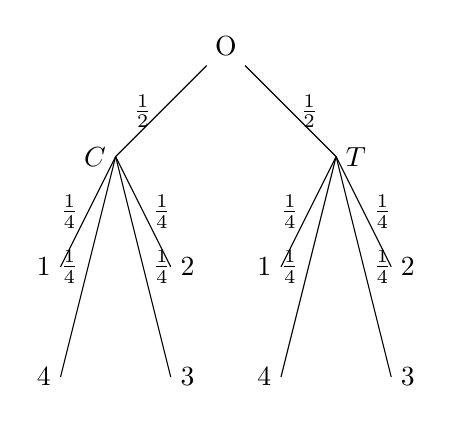
\begin{tikzpicture}[scale=0.7]
    \node (root) at (0,0) {O};
    \draw (root) -- (-2,-2) node[left] {$C$} node[midway,left] {$\frac{1}{2}$};
    \draw (root) -- (2,-2) node[right] {$T$} node[midway,right] {$\frac{1}{2}$};
    
    \draw (-2,-2) -- (-3,-4) node[left] {$1$} node[midway,left] {$\frac{1}{4}$};
    \draw (-2,-2) -- (-1,-4) node[right] {$2$} node[midway,right] {$\frac{1}{4}$};
    \draw (-2,-2) -- (-1,-6) node[right] {$3$} node[midway,right] {$\frac{1}{4}$};
    \draw (-2,-2) -- (-3,-6) node[left] {$4$} node[midway,left] {$\frac{1}{4}$};
    
    \draw (2,-2) -- (1,-4) node[left] {$1$} node[midway,left] {$\frac{1}{4}$};
    \draw (2,-2) -- (3,-4) node[right] {$2$} node[midway,right] {$\frac{1}{4}$};
    \draw (2,-2) -- (3,-6) node[right] {$3$} node[midway,right] {$\frac{1}{4}$};
    \draw (2,-2) -- (1,-6) node[left] {$4$} node[midway,left] {$\frac{1}{4}$};
\end{tikzpicture}

  \[
  \begin{aligned}
    & T = \text{"esito del lancio moneta e testa"} \\
    & C = \text{"esito del lancio moneta è croce"} \\
    & D_i = \text{"è uscito il numero } i \text{"} \\
    & P(C) = \frac{1}{2}, \quad P(T) = \frac{1}{2} \\
    & P(D_i | C) = \frac{1}{4} \\
    & P(D_i | T) = \frac{1}{4} \\
    & A = \text{"è uscito testa e il numero } i \text{"} \\
    & P(A) = P(T) \cdot P(D_i | T) = \frac{1}{2} \cdot \frac{1}{4} = \frac{1}{8} \\
    & \text{Analogamente per } C \cap D_i
  \end{aligned}
  \]
}

\ex{Esempio}{
  Nel 
}

\subsection{Formula di Boyes}
Quando si deve calcolare una probabilità condizionata di eventi "nell'ordine temporale sbagliato", ad esempio se si calcolare $P(A|B)$ ma si conosce solo $P(B|A)$, si può utilizzare uno strumento utilissimo facilmente derivabile dalla matematica della probabilità condizionata, ovvero la formula di Bayes:

\thm{Formula di Bayes}{
  Siano $A$ e $B$ due eventi tali che $\mathbb{P}(A)>0$ e $\mathbb{P}(B)>0$, allora:
  \[
    \mathbb{P}(A|B) = \frac{\mathbb{P}(B|A)\mathbb{P}(A)}{\mathbb{P}(B)}
  \]
}
\pf{Dimostrazione}{

  Per definizione di $\mathbb{P}(A|B)$ si ha:
  \[
    \mathbb{P}(A|B) = \frac{\mathbb{P}(A \cap B)}{\mathbb{P}(B)}
  \]
  Utilizzando la regola della catena possiamo rimuovere il numeratore come segue:
  \[
    \mathbb{P}(A\cap B) = \mathbb{P}(B|A)\mathbb{P}(A)
  \]
  Quindi:
  \[
    \mathbb{P}(A|B) = \frac{\mathbb{P}(A \cap B)}{\mathbb{P}(B)} = \frac{\mathbb{P}(B|A)\mathbb{P}(A)}{\mathbb{P}(B)}
  \]
}

\ex{}{
  Ci sono due urne: la prima urna contiene una pallina bianca e due palline
rosse, mentre la seconda contiene due palline bianche e cinque palline rosse. Si lancia una
moneta: se esce testa si estrae una pallina dalla prima urna, se esce croce si estrae una
pallina dalla seconda.
Sapendo che è stata estratta una pallina bianca, calcolare la probabilità che l’esito del
lancio della moneta sia stato testa.

Svolgimento:

$T = \text{"esce testa"}$
}

% \end{document}

\begin{document}
\chapter{Calcolo Combinatorio}  

Quando abbiamo numero finito di elementi, e' possibile contare gli elementi dell'evento per ridurre il problema di probabilita' a un problema di conteggio -> dobbiamo imparare a contare

Dato un certo insieme, dobbiamo calcolarne la cardinalita' utilizzando i giusti stumenti matematici

\thm{Calcolo probabilita' uniforme (Laplace)}{
  Se $ \Omega $ e' finito, $ \Omega = \{w_1,...,w_N\} $ e $ \forall i = 1,...,N.\ \mathbb{P}(\{w_i\}) = \frac{1}{N} $ (probabilita' uniforme), allora $ \forall A \subseteq \Omega $ (evento):
  \[
    \mathbb{P}(A) = \frac{|A|}{N}
  \]
}

Dobbiamo introdurre:
\begin{itemize}
\item \textbf{Fattoriali}:
  \begin{itemize}
  \item $ 0! \coloneq 1 $
  \item $ (n+1)! \coloneq (n+1) \cdot n! $
  \end{itemize}
  \item \textbf{Coefficenti Binomiali}:
    \[
      (n,k) = \frac{n!}{k! (n-k)!} \quad \forall n,k\in \mathbb{N}. n \geq k
    \]
    In generale:
    \[
      (n,k) = (n,n-k)
    \]
    Dal triangolo di Tartaglia, possiamo visualizzare altre proprieta' (oltre alla simmetria)
\end{itemize}

Vedremo che $ (n,k) $ sono il numero di modi diversi che abbiamo per selezionare $ k $ sottoinsiemi diversi da un insieme di cardinalita' $ n $.

\thm{Formula di Newton}{
  \[
    (a+b)^n = \sum_{k=0}^{n} (n,k) a^k b^{n-k}
  \]
}

Quindi anche il coefficente deriva da un problema di conteggio.

\section{Metodo (Principio) delle Scelte Successive}
E' un algoritmo per determinare la cardinalita' di un insieme. Vediamo un esempio:
\ex{}{
  Alfabeto di 36 caratteri dove ognuno dei numeri corrisponde a un carattere alfanumerico.

  \underline{Domanda}: "Quante possibili password distinte di 8 caratteri esistono in questo alfabeto?"

  $ \Omega = \text{Alfanumerici} \times ... \times \text{Alfanumerici} $ 8 volte.

  \begin{itemize}
  \item Scelte:
    \begin{enumerate}
    \item un carattere dei 36 totali
    \item \vdots (e' cosi 8 volte)
    \end{enumerate}
    Quindi $ |\Omega| = 36 \times ... \times 36 = 36^8 $
  \end{itemize}

  E se vogliamo evitare di ripetere i caratteri? Vediamo le scelte:
  \begin{enumerate}
  \item un carattere dei 36 totali
  \item un carattere dei \textbf{35 possibili}
  \item \vdots
  \item un carattere dei 29 possibili
  \end{enumerate}
  Quindi $ |\Omega| = 36 \times 35 \times ... \times 29 = \frac{36!}{28!} $
}

Definiamo il principio generale:

\thm{Non proprio un teorema}{
  Ciascun elemetno di un insieme $ A $ puo' essere determinato tramite sola sequenza di $ k $ scelte, dove per ogni scelta ci sono $ n_1,....,n_k $ possibilita', allora:
  \[
  |A| = n_1 \times ... \times n_k
  \]
}

\nt{
  Puo' essere riscritto come teorema formale ma \textbf{E' TROPPO DIFFICILE PER NOI INFORMATICI} quindi non lo facciamo!!!!
}

\ex{}{
  52 carte (13 tipi 4 semi)
  \begin{enumerate}
    \item $ A = \text{iniseme dei full (un tris e una coppia)} $, $ |A| = ? $

      \underline{4 scelte:}
      \begin{itemize}
        \item tipo di carta nel tris (13)
        \item tipo di carta nella coppia (12)
        \item semi nel tris (4)
        \item semi nella coppia (6)
      \end{itemize}
      $ |A| = 13 12 4 6 = \text{casi favorevoli} $

    \item $ A = \text{doppie coppie (due coppie di tipo diverso e una carta libera)} $, $ |A|=? $

      \underline{Scelte}:
      \begin{itemize}
        \item tipo nella prima coppia (13)
        \item tipo nella seconda coppia (12)
        \item semi nella prima coppia (6)
        \item semi seconda (6)
        \item tipo singolo (11)
        \item seme singolo (4)
      \end{itemize}
      $ |A| = 13 12 6 6 11 4 $ \textbf{SBAGLIATO!!}

      Perche' non ci interessa dell'ordine delle due coppie (bisogna dedurlo dalla definizione di A), quindi NON c'e' una prima e seconda coppia (anche sopra era sbagliato vederlo cosi') dato che non c'e' l'ordine.

      Combinazioni dei tipi che compongono 2 coppie ($ 13 \times 12 / 2 $)
  \end{enumerate}
}

\section{Disposizioni e Combinazioni}

\def{Disposizioni con ripetizione}{
  Dato un insieme $ E $ con $ n $ elementi, indichiamo con $ DR_{n,k} $ le sequenze ordinate di $ k $ elementi di $ E $. 
}
Sostanzialmente, $ DR_{n,k} = E \times E ... \times E $ $ k $ volte, ovvero:
\[
DR_{n,k} = E^k
\]
Quindi usando il principio delle scelte successive:
\[
|DR_{n,k}| = n^k
\]
dato che per ogni $ E $ abbiamo una scelta fra $ n $ elementi.

\nt{
  Indicando tale insieme con $ DR_{n,k} $, l'insieme $ E $ sparisce, dato che ci interessa solo la \textbf{cardinalita'} di tale insieme e non ce ne frega un cavolo dei sui elementi.
}

\ex{Iniziamo a calcolare le probabilita'!}{
  Presa un urna con $ n $ palline numerate ($ E = \{1,...,n\} $) e si estraggono $ k $ palline con \textit{reinbussolamento}.
  \[
  \Omega = E \times ... \times E = DR_{n,k}
  \]
  Quindi $ |\Omega| = n^k $, e la probabilita' uniforme e' data da:
  \[
    \mathbb{P}(\{\omega\}) = \frac{1}{|\Omega|} = n^{-k}
  \]
}
\ex{}{
  Determinare spazi campionari per i seguenti esperimenti:
  \begin{itemize}
  \item Scelta casuale di una parola di 8 lettere
  \item Scelta di colonne deltotocalcio (risultato di 13 partite)
  \end{itemize}
}

Quindi lo usiamo nei casi di estrazione con reinbussolamento quando ci interessa l'ordine.

\def{Disposizioni}{
  Dato un insieme $ E  $ di $ n $ elementi, l'insieme delle disposizioni (senza ripetizione) di $ k $ elementi dell'insieme $ E $ e' l'insieme delle sequenze ordinate di $ k $ elementi \textit{distinti}, ovvero:
  \[
    D_{n,k} \coloneq \{(x_1,...,x_k)|x_1,...,x_k \in E \land x_i \neq x_j \text{se} i \neq j \}
  \]
}

\nt{
  $ D_{n,k} $ e' un sottoinsieme \textbf{stretto} di $ DR_{n,k} $.
}

Usando le scelte successive:
\[
  |D_{n,k}| = n\times (n-1) \times ... \times (n-k+1) = \frac{n!}{(n-k)!}
\]
L'esperimento aleatorio di riferimento e' l'estrazione \textbf{senze} reimissione.

\dfn{Permutazioni}{
  $ P_n = D_{n,n} $, quindi:
  $ |P_n| = n! $
}

\dfn{}{
  Dato un insieme $ E $ di $ n $ elementi, indichiamo con $ C_{n,k} $ la classe dei sottoinsiemi di $ E $ contenenti $ k $ elementi, ovvero:
  \[
  C_{n,k} = \{A \subseteq E | |A|= k\}
  \]
}
Siamo passati da sequenze a sottoinsiemi, ovvero non ci interessa piu' dell'ordine:
\[
\text{sottoinsieme} = \text{sequenza non ordinata}
\]

\end{document}


% \begin{document}
\chapter{Esercitazione}
%%%%%%%%%%%%%%%%%%%%%%%%%%%%%%%%%%%%%%%%%%%%%%%%%%%%%%%%%%%%%%%%%%%%%%%%%%%%%%%
% Esercizio 4 (Foglio 2)
%%%%%%%%%%%%%%%%%%%%%%%%%%%%%%%%%%%%%%%%%%%%%%%%%%%%%%%%%%%%%%%%%%%%%%%%%%%%%%%

\section{Esercitazione 4/03}
\subsection{Esercizio 4 (Foglio 2)}
\subsubsection{Testo}
Un’urna contiene \(r\) palline rosse e \(b\) palline bianche. Si eseguono due estrazioni senza reimmissione.
\begin{enumerate}[label=(\alph*)]
    \item Determinare uno spazio di probabilità che descriva l’esperimento aleatorio.
    \item Calcolare la probabilità che la prima pallina estratta sia rossa.
    \item Calcolare la probabilità che la prima pallina sia rossa e la seconda bianca.
    \item Calcolare la probabilità che le due palline abbiano colori diversi.
    \item Calcolare la probabilità che la seconda pallina estratta sia rossa.
\end{enumerate}

\subsubsection{Soluzione}
Siano:

$R_i$ = "ho estratto una pallina rossa all'i-esima iterazione"
$B_i$ = "ho estratto una pallina rossa all'i-esima iterazione"

Definiamo lo spazio degli esiti. Poiché le estrazioni avvengono senza reimmissione, ogni esito è una coppia ordinata di palline diverse. Denotiamo:
\[
    \Omega = \{ (p_1, p_2) : p_1, p_2 \text{ sono palline dell'urna e } p_1 \neq p_2 \}
\]
La cardinalità totale è:
\[
    |\Omega| = (r+b)(r+b-1)
\]
Infatti appena estraiamo una pallina l'urna conterrà $(r+b-1)$ palline, la totalità di palline -1

Sfruttiamo il principio di probabilità uniforme, secondo cui ogni esito ha probabilità \(1/|\Omega|\)

\begin{enumerate}[label=(\alph*)]
    \item \textbf{Spazio di probabilità:}\\
    Lo spazio di probabilità è \((\Omega, P)\) con
    \[
        P(\{ \omega \}) = \frac{1}{(r+b)(r+b-1)} \quad \forall \omega \in \Omega.
    \]
    
    \item \textbf{Probabilità che la prima pallina sia rossa:}\\[1mm]
    Poiché ci sono \(r\) palline rosse su un totale di \(r+b\), si ha:
    \[
        P(R_1) = \frac{r}{r+b}.
    \]
    
    \item \textbf{Probabilità che la prima pallina sia rossa e la seconda bianca:}\\[1mm]
    Dato che la prima è rossa, nell’urna rimangono \(r+b-1\) palline, di cui \(b\) sono bianche:
    \[
        P(R_1 \cap B_2) = P(B_2 | R_1) P(R_1) =\frac{r}{r+b} \cdot \frac{b}{r+b-1}.
    \]
    
    \item \textbf{Probabilità che le due palline abbiano colori diversi:}\\[1mm]
    Questa condizione si verifica in due modi: rossa poi bianca oppure bianca poi rossa. Quindi:
    \[
        \begin{split}
            P((R_1 \cap B_2)\cup (B_1 \cap R_2)) & =P(B_2 | R_1) P(R_1) + P(R_2 | B_1) P(B_1)\\
                    &= \frac{r}{r+b} \cdot \frac{b}{r+b-1} + \frac{b}{r+b} \cdot \frac{r}{r+b-1} \\
                    &= \frac{2rb}{(r+b)(r+b-1)}.
        \end{split}
    \]
    \item \textbf{Probabilità che la seconda pallina sia rossa:}\\[1mm]
    Usiamo la formula della probabilità totale, considerando le possibili estrazioni del primo turno:
    \[
    \begin{split}
    P(R_2) &= P(B_2 \mid R_1) \cdot P(R_1)  + P(B_2 \mid B_1) \cdot P(B_1)\\[1mm]
    &= \frac{r-1}{r+b-1} \cdot \frac{r}{r+b} + \frac{r}{r+b-1} \cdot \frac{b}{r+b}
    \end{split}
    \]
    Semplificando:
    \[
    P(R_2) = \frac{r(r-1) + rb}{(r+b)(r+b-1)} = \frac{r^2 - r + rb}{(r+b)(r+b-1)} = \frac{r(r+b-1)}{(r+b)(r+b-1)} = \frac{r}{r+b}
    \]
\end{enumerate}

\subsubsection{Esercizio 6}
\subsubsection{Testo}
Supponiamo che un’urna contenga 1 pallina rossa e 1 pallina bianca. Una pallina viene estratta e se ne osserva il colore. La pallina estratta viene poi rimessa nell’urna insieme a un’altra pallina dello stesso colore (estrazione con rinforzo). Siano
\[
\begin{aligned}
    R_i &= \text{evento che all'}i\text{-esima estrazione venga estratta una pallina rossa,}\\
    B_i &= \text{evento che all'}i\text{-esima estrazione venga estratta una pallina bianca.}
\end{aligned}
\]
Si calcolino:
\begin{enumerate}[label=(\arabic*)]
    \item \(P(R_2)\)
    \item Sapendo che la seconda pallina estratta è rossa, quale è l’evento più probabile per la prima estrazione: che la pallina estratta sia stata rossa oppure bianca?
\end{enumerate}

\subsubsection{Soluzione}
\begin{enumerate}[label=(\arabic*)]
    \item \textbf{Calcolo di \(P(R_2)\):}\\[1mm]
    \textbf{Caso 1:} Se alla prima estrazione esce una pallina rossa (evento \(R_1\)):
    \begin{itemize}
        \item La probabilità di estrarre una rossa al primo turno è \(P(R_1)=\frac{1}{2}\).
        \item Dopo l’estrazione, la pallina rossa viene rimessa insieme a un’altra rossa, dunque l’urna contiene 2 rosse e 1 bianca. Quindi:
        \[
        P(R_2 \mid R_1)=\frac{2}{3}.
        \]
    \end{itemize}
    \textbf{Caso 2:} Se alla prima estrazione esce una pallina bianca (evento \(B_1\)):
    \begin{itemize}
        \item \(P(B_1)=\frac{1}{2}\).
        \item Dopo il rinforzo, l’urna contiene 1 rossa e 2 bianche, dunque:
        \[
        P(R_2 \mid B_1)=\frac{1}{3}.
        \]
    \end{itemize}
    Applicando la formula della probabilità totale:
    \[
    \begin{split}
    P(R_2) &= P(R_2 \mid R_1) \cdot P(R_1) + P(R_2 \mid B_1) \cdot P(B_1) \\
    &= \frac{2}{3}\cdot\frac{1}{2} + \frac{1}{3}\cdot\frac{1}{2} \\
    &= \frac{1}{3} + \frac{1}{6} = \frac{1}{2}.
    \end{split}
    \]
    
    \item \textbf{Confronto tra \(P(R_1 \mid R_2)\) e \(P(B_1 \mid R_2)\):}\\[1mm]
    
    Innanzi tutto si tenga conto il teorema di Bayes:\\ 
    Siano $A,B$ due eventi, t.c. $P(A), P(B)>0$, allora $P(A\mid B) = \frac{P(B\mid A) P(A)}{P(B)}$

    Dimostrazione: 
    Abbiamo $P(A\cap B) = P(B\cap A)$, quindi $P(A\mid B) = \frac{P(A\cap B)}{P(B)} = \frac{P(B\mid A)P(A)}{P(B)}$


    Usiamo il teorema di Bayes per calcolare \(P(R_1 \mid R_2)\):
    \[
    P(R_1 \mid R_2) = \frac{P(R_2 \mid R_1) \, P(R_1)}{P(R_2)} 
    = \frac{\frac{2}{3} \cdot \frac{1}{2}}{\frac{1}{2}}
    = \frac{2}{3}.
    \]
    Poiché \(P(B_1 \mid R_2) =1- P(B_1^c \mid R_2) =1 - P(R_1 \mid R_2) = 1 - \frac{2}{3} = \frac{1}{3}\), risulta che,
    \[
    P(R_1 \mid R_2) > P(B_1 \mid R_2).
    \]
    Quindi, sapendo che la seconda pallina è rossa, è più probabile che la prima pallina estratta fosse rossa.
\end{enumerate}


\subsection{Esercizio 7}
\subsubsection{Testo}
Si consideri una popolazione in cui una persona su 100 abbia una certa malattia. Un test è disponibile per diagnosticare tale malattia. Si supponga che il test non sia perfetto, in quanto esso risulta positivo (ovvero indica la presenza della malattia) nel 5\% dei casi quando è effettuato su persone sane, mentre risulta negativo (indicando l’assenza della malattia) nel 2\% dei casi quando è effettuato su persone malate. Si calcolino le probabilità che:
\begin{enumerate}[label=(\alph*)]
    \item il test risulti positivo quando effettuato su una persona malata,
    \item il test risulti positivo,
    \item una persona sia malata se il test risulta positivo.
\end{enumerate}

\subsubsection{Soluzione}
I dati del problema sono: 
\begin{itemize}
    \item \(P(M)=0.01\): probabilità che una persona sia malata.
    \item \(P(S)=0.99\): probabilità che una persona sia sana.
    \item \(P(T^+ \mid M)=0.98\): probabilità che il test risulti positivo se la persona è malata.
    \item \(P(T^- \mid M)=0.02\): probabilità che il test risulti negativo se la persona è malata.
    \item \(P(T^+ \mid S)=0.05\): probabilità che il test risulti positivo se la persona è sana.
    \item \(P(T^- \mid S)=0.95\): probabilità che il test risulti negativo se la persona è sana.
\end{itemize}


Costruiamo un diagramma di verità:
\begin{center}
    \begin{tabular}{|c|c|c|}
        \hline
        & Malato & Sano \\
        \hline
        Positivo & 0.98 & 0.05 \\
        \hline
        Negativo & 0.02 & 0.95 \\
        \hline
    \end{tabular}
\end{center}


\begin{enumerate}
    \item \textbf{Probabilità che il test risulti positivo su una persona malata}: Questa probabilità è data direttamente dai dati:
    \[
        P(T^+ \mid M)=0.98.
    \]
    
    \item \textbf{Probabilità che il test risulti positivo}:Utilizziamo la formula della probabilità totale:
    \[
    \begin{split}
    P(T^+) &= P(T^+ \mid M) \, P(M) + P(T^+ \mid S) \, P(S) \\
    &= 0.98 \cdot 0.01 + 0.05 \cdot 0.99 \\
    &= 0.0098 + 0.0495 \\
    &\approx 0.0593.
    \end{split}
    \]
    
    \item \textbf{Probabilità che una persona sia malata, dato un test positivo:}\\[1mm]
    Applichiamo il teorema di Bayes:
    \[
    \begin{split}
    P(M \mid T^+) &= \frac{P(T^+ \mid M) \, P(M)}{P(T^+)} \\
    &= \frac{0.98 \cdot 0.01}{0.0593} \\
    &\approx \frac{0.0098}{0.0593} \\
    &\approx 0.165.
    \end{split}
    \]
    Quindi, circa il 16,5\% delle persone con test positivo sono effettivamente malate.    
\end{enumerate}

\subsection{Esercizio 5}
\subsubsection{Testo}
Si consideri il seguente esperimento:

    ci sono quattro dadi: due non truccati e due truccati. I dadi truccati hanno tre facce con il numero \(6\) e tre facce con il numero \(5\). Si lancia una moneta (non truccata). Se viene \emph{testa} si lanciano i due dadi non truccati, mentre se viene \emph{croce} si lanciano i due dadi truccati.

Si richiede di calcolare:
\begin{enumerate}[label=(\alph*)]
    \item La probabilità che la somma dei due dadi sia \(11\).
    \item Sapendo di aver ottenuto \(11\) dalla somma dei due dadi, calcolare la probabilità che il lancio della moneta sia stato \emph{croce}.
\end{enumerate}

\subsubsection{Soluzione}
\begin{tikzpicture}
  [
    grow                    = right,
    sibling distance        = 8em,
    level distance          = 8em,
    edge from parent/.style = {draw, -latex},
    every node/.style       = {font=\footnotesize},
    sloped
  ]
  
  \node {$\Omega$}
    child { node {Testa ($\frac{1}{2}$)}
      child { node {Dado 1}
        child { node {1,2,3,4,5,6 ($\frac{1}{6}$)}} 
      }
      child { node {Dado 2}
        child { node {1,2,3,4,5,6 ($\frac{1}{6}$)}} 
      }
    }
    child { node {Croce ($\frac{1}{2}$)}
      child { node {Dado 1}
        child { node {5 ($\frac{1}{2}$)}}
        child { node {6 ($\frac{1}{2}$)}}
      }
      child { node {Dado 2}
        child { node {5 ($\frac{1}{2}$)}}
        child { node {6 ($\frac{1}{2}$)}}
      }
    };
\end{tikzpicture}

Sia:
\[
T = \{\text{moneta: testa}\}, \quad C = \{\text{moneta: croce}\},
\]
con \(P(T)=P(C)=\frac{1}{2}\).

\textbf{Caso 1: Dadi non truccati (se esce testa)}\\[1mm]
I dadi non truccati hanno facce \(1,2,3,4,5,6\) con probabilità uniforme. La somma \(11\) si ottiene con le coppie \((5,6)\) e \((6,5)\). Quindi:
\[
P(11 \mid T) = \frac{2}{36} = \frac{1}{18}.
\]

\textbf{Caso 2: Dadi truccati (se esce croce)}\\[1mm]
I dadi truccati assumono solo i valori \(5\) e \(6\) con probabilità \( \frac{3}{6} = \frac{1}{2}\) ciascuno. La somma \(11\) si ottiene con le coppie \((5,6)\) e \((6,5)\), dunque:
\[
P(11 \mid C) = 2 \cdot \left(\frac{1}{2} \cdot \frac{1}{2}\right) = \frac{1}{2}.
\]

\textbf{Calcolo della probabilità totale di ottenere \(11\):}
\[
\begin{split}
P(11) &= P(11 \mid T) \, P(T) + P(11 \mid C) \, P(C) \\
&= \frac{1}{18} \cdot \frac{1}{2} + \frac{1}{2} \cdot \frac{1}{2} \\
&= \frac{1}{36} + \frac{1}{4} = \frac{1}{36} + \frac{9}{36} = \frac{10}{36} = \frac{5}{18}.
\end{split}
\]

\textbf{Calcolo della probabilità condizionata \(P(C \mid 11)\):}
Utilizzando il teorema di Bayes:
\[
P(C \mid 11) = \frac{P(11 \mid C) \, P(C)}{P(11)} 
= \frac{\frac{1}{2} \cdot \frac{1}{2}}{\frac{5}{18}} 
= \frac{\frac{1}{4}}{\frac{5}{18}} 
= \frac{1}{4} \cdot \frac{18}{5} 
= \frac{9}{10}.
\]
Quindi, se la somma è \(11\), la probabilità che la moneta abbia dato \emph{croce} è \(\frac{9}{10}\).

\subsection{Esercizio 2}
\subsubsection{Testo}

Si consideri l’esperimento di lanciare due volte un dado.
\begin{enumerate}[label=(\alph*)]
\item Determinare uno spazio di probabilit‘a che descriva l’esperimento aleatorio.
  \item Si considerino i seguenti eventi:
\begin{itemize}
\item A = “numero dispari sul primo dado”
\item B =“numero dispari sul secondo dado”
\item C = “la somma dei due risultati ‘e dispari”
\end{itemize}
Gli eventi A, B e C sono indipendenti?
\item Si considerino ora gli eventi:
  \begin{itemize}
  \item E = “il risultato del secondo lancio ‘e 1, 2 o 5”
    \item F = “il risultato del secondo lancio ‘e 4, 5 o 6”
    \item G = “la somma dei due risultati ‘e 9”
  \end{itemize}
  Gli eventi E, F e G sono indipendenti?
\end{enumerate}

\subsubsection{Soluzione}

\begin{enumerate}[label=(\alph*)]
  \item $ (\Omega, \mathbb{P}) = ? $:
    \begin{itemize}
    \item $ \Omega = \{1,...,6\} \times \{1,...,6\} $
    \item I due sottoesperimenti sono indipendenti e hanno probabilita' uniforme, quindi:
      \begin{align*}
        \mathbb{P}((x_1, x_2)) &= \mathbb{P}(x_1)\mathbb{P}(x_2)\\
        &= \frac{1}{6}\frac{1}{6}\\
        &= \frac{1}{36}\\
        &= \frac{1}{|\Omega|}
      \end{align*}
        Quindi anche l'esperimento principale ha probabilita' uniforme.
    \end{itemize}
  \item Dimostriamo per controprova che $ A,B $ e $ C $ non sono indipendenti:
    \begin{align*}
      \mathbb{P}(A \cap B \cap C) &= \mathbb{P}(A)\mathbb{P}(B|A)\mathbb{P}(C|A \cap B)\\
      &= \frac{1}{2}\frac{1}{2}0\\
      &= 0 \neq \mathbb{P}(A)\mathbb{P}(B)\mathbb{P}(C) (\text{dato che e' sicuramente }> 0)
    \end{align*}
  \item Dimostriamo per controprova che $ D,E $ e $ F $ non sono indipendenti;
    \begin{align*}
      \mathbb{P}(E|F) &= \frac{\mathbb{P}(E \cap F)}{\mathbb{P}(F)}\\
      &= \frac{1}{3} \neq \mathbb{P}(E) (=\frac{1}{2})
    \end{align*}
\end{enumerate}

\subsection{Esercizio 3}
\subsubsection{Testo}

I componenti prodotti da una ditta possono avere due tipi di difetti con percentuali del 3\% e del 7\% rispettivamente
e in modo indipendente l’uno dall’altro. Qual ‘e la probabilit‘a che un componente scelto a caso
\begin{enumerate}[label=(\alph*)]
\item presenti entrambi i difetti?
\item sia difettoso?
\item presenti il primo difetto, sapendo che ‘e difettoso?
\item presenti uno solo dei difetti, sapendo che ‘e difettoso?
\end{enumerate}

\subsubsection{Soluzione}

$ D_1 = \text{"prodotto presenta il difetto 1"} $

$ D_2 = \text{"prodotto presenta il difetto 2"} $
\begin{enumerate}[label=(\alph*)]
  \item $ \mathbb{P}(D_1 \cap D_2) = ? $ dato che non ci viene detto niente, possiamo ipotizzare che gli eventi sono indipendenti, quindi:
    \begin{align*}
      \mathbb{P}(D_1 \cap D_2) &= \mathbb{P}(D_1)\mathbb{P}(D_2)\\
      &= \mathbb{P}(D_1)\mathbb{P}(D_2)\\
      &= 0.03 \cdot 0.07
    \end{align*}
  \item $ \mathbb{P}(D_1 \cup D_2) = ? $ proviamo a usare DeMorgan, tenendo in mente che i complementari di eventi indipendenti sono anch'essi indipendenti:
    \begin{align*}
      \mathbb{P}(D_1 \cup D_2) &= 1 - \mathbb{P}(D_1^{c} \cap D_2^{c})\\
      &= 1 - \mathbb{P}(D_1^{c})\mathbb{P}(D_2^{c})\\
      &= 1 - 0.97\cdot 0.93
    \end{align*}
  \item $ \mathbb{P}(D_1 | D_1 \cup D_2) = ? $ possiamo usare Bayes e il risultato trovato nel punto prima:
    \begin{align*}
      \mathbb{P}(D_1 | D_1 \cup D_2) &= \frac{\mathbb{P}(D_1 \cup D_2 | D_1)\mathbb{P}(D_1)}{\mathbb{P}(D_1 \cup D_2)}\\
      &= \frac{1\cdot 0.03}{1 - 0.97\cdot 0.93}
    \end{align*}
  \item $ \mathbb{P}((D_1 \cap D_2^{c})\cup(D_1^{c} \cap D_2) | D_1 \cup D_2) = ? $
    \begin{align*}
      \mathbb{P}((D_1 \cap D_2^{c}) \cup (D_1^{c} \cap D_2) | D_1 \cup D_2) &= \frac{\mathbb{P}(D_1 \cup D_2 | (D_1 \cap D_2^{c})\cup (D_1^{c} \cap D_2))\mathbb{P}((D_1 \cap D_2^{c})\cup(D_1^{c} \cap D_2))}{\mathbb{P}(D_1 \cup D_2)}\\
      &= \frac{1 \cdot \mathbb{P}((D_1 \cap D_2^{c})\cup(D_1^{c} \cap D_2))}{\mathbb{P}(D_1 \cup D_2)}
    \end{align*}
    Ci rimane quindi da calcolare la probabilita al numeratore. Notare che:
    \begin{align*}
      (D_1 \cap D_2^{c}) \cap (D_1^{c} \cap D_2) &= D_1 \cap D_2^{c} \cap D_1^{c} \cap D_2\\
      &= D_1 \cap D_1^{c} \cap D_2 \cap D_2^{c}\\
      &= \emptyset
    \end{align*}
    Quindi, essendo eventi disgiunti possiamo applicare l'addittivita' finita:
    \begin{align*}
      \mathbb{P}((D_1 \cap D_2^{c}) \cup (D_1^{c} \cap D_2)) &= \mathbb{P}(D_1 \cap D_2^{c})+\mathbb{P}(D_1^{c} \cap D_2)\\
      &= \mathbb{P}(D_1)\mathbb{P}(D_2^{c}) + \mathbb{P}(D_1^{c})\mathbb{P}(D_2)
    \end{align*}
\end{enumerate}

\subsection{Esercizio Porco Rosso}
\subsubsection{Testo}

L’aereo dei pirati del cielo, appena riparato, è stato dato alle fiamme. Porco Rosso vuole scoprire chi è stato. Durante le indagini si è scoperto che la settimana prima del delitto i pirati del cielo hanno detto al meccanico della ditta Piccolo che non gli avrebbero pagato la riparazione dell’idrovolante. Interrogato da Porco Rosso, Piccolo cerca di scagionarsi dicendo che a seguito di insolvenza solo 1 meccanico su 1000 si vendica. Porco Rosso però si accorge che questa stima non è più significativa: bisogna valutare la probabilità di vendetta sapendo che l’aereo è stato effettivamente dato alle fiamme. Porco Rosso allora considera questi eventi:

\begin{itemize}
    \item \(A\): dei clienti risultano insolventi contro il proprio meccanico,
    \item \(B\): l’aereo di un cliente viene distrutto dal meccanico,
    \item \(C\): l’aereo di un cliente viene distrutto ma non dal proprio meccanico.
\end{itemize}

A questo punto è necessario il vostro aiuto!

\begin{enumerate}[label=(\alph*)]
    \item Esprimere in funzione di \(A\), \(B\) e \(C\) la probabilità fornita da Piccolo e calcolarla.
    \item Quali eventi tra \(A\), \(B\) e \(C\) possono essere ritenuti disgiunti?
    \item Quali eventi tra \(A\), \(B\) e \(C\) possono essere ritenuti indipendenti?
    \item Esprimere in funzione di \(A\), \(B\) e \(C\) l’evento \(D\): l’aereo di un cliente viene distrutto.
    \item Esprimere la probabilità condizionata \(P(B|A \cap D)\) in funzione solo di \(P(B|A)\) e \(P(C)\).
    Porco Rosso non riesce a trovare \(P(C)\), tuttavia trova che 1 aereo ogni 10000 viene distrutto.
    \item Limitare (dal basso o dall’alto) il valore di \(P(B|A \cap D)\).
    \item È il caso che Porco Rosso continui ad indagare su Piccolo?
\end{enumerate}

\subsubsection{Soluzione}
\begin{itemize}
    \item $P(B|A) = \frac{1}{1000} = \frac{P(A\cap B)}{P(A)}$, 
    \item $B\cap C = \emptyset$
    \item Quali tra A,B,C   sono indipendenti? $P(A\cap B) = P(A)\cdot P(B)$, $P(A\cap C) = P(A)\cdot P(C)$
    \item D = "Areo distrutto" = $B\cup C$
    \item $P(B | A\cap D)$ sono in funzione di $P(B|A)$ e $P(C)$, quindi $= \frac{B\cap A \cap D}{P(A\cap D)} = \frac{B\cap A\cap (B \sqcup C)}{ P(A\cap (B\sqcup C))} = \frac{((B\cap A))}{P(A \cap (B \cup C))} $
\end{itemize}

\subsection{Esercizio 2.3}
\subsubsection{Testo}
Nel gioco del lotto si estraggono senza reimmissione cinque numeri da un'unrna che contiene 90 palline da 1 a 9
\begin{enumerate}
    \item Determinare una spazio di probabilità che descriva l'esperimento aleatorio
    \item Come cambia la risposta al punto precedente se le estrazioni avvengono con reimmissione?
\end{enumerate}

\subsubsection{Svolgimento}
\begin{enumerate}
    \item \begin{itemize}
        \item  $\Omega = \{(x_1, x_2, x_3, x_4,_5)\mid x_i\in \{1,\dots, 90\}, i=1,\dots,5, x_i \text{ distinti}\}$
        \item .
        Definisco:

        $\forall i\in\{1,\dots, 5\} \forall j\in \{1,\dots, 90\},\, E_{ij}:$ "straggo il numero $j$ all'i-esima estrazione" 

        $\mathbb{P}(E_{1,x_1}\cap E_{2,x_3}\cap E_{3,x_3}\cap E_{4,x_4}\cap E_{5,x_5})= \mathbb{P} (E_{1,x_1}) \mathbb{P}(E_{2,x_2}|E_{1,x_1}) \dots \mathbb{P}(E_{5,x_5} | E_{1,x_1}\cap E_{2,x_2}\cap E_{3,x_3} \cap E_{4,x_4} \cap E_{5,x_5})$ assumo che vi è probabilità uniforme $= \frac{1}{90}\cdot\frac{1}{89}\cdot \frac{1}{88}\cdot\frac{1}{87}\cdot\frac{1}{86} = \frac{1}{|\Omega|}$
    \end{itemize}
    
   

    \item $\Omega = \{(x_1, x_2, x_3, x_4,_5)\mid x_i\in \{1,\dots, 90\}, i=1,\dots,5\}$
    
    sotto-esperimento: estrazione dall'urna, dato che avviene la reimmissione si ha che ogni sotto-esperimento è indipendente, quindi si ha:
    \[
        \mathbb{P}(\cdot) \text{ uniforme per }\Omega: \mathbb{P}(\omega)
    \]
\end{enumerate}

\subsection{}
\subsubsection{Testo}
Un'urna contiene 10 palline di cui 6 bianche e 4 rosse. Si estraggono due palline senza reimmissione. Calcolare la probabilità dell'evento

\[
    B_2 =\text{ la seconda è bianca }
\]

\subsubsection{Svolgimento}
Sia $B_i = $"estraggo una pallina bianfa all'i-esima estrazione"

$\mathbb{P}(B_2)$?

TODO: giaga alberello

Formula delle porb totali:
\[
    \mathbb{P}(B_2) = P(B_2 \cap B_1) + P(B_2\cap B_1^c )= P(B_2| B_1)P (B_1)  P(B_2| B_1^c)P (B_1^c) +  = \frac{5}{9}\cdot \frac{6}{10}+\frac{6}{9}\cdot\frac{4}{10}
\]


\end{document}
